% Core.Tex, version=13
% Satin Dmitri, 2016-2018

% Changelog:
% 13: Add No Title mode
% 12.1: Improve \N, \Q, \R, \Z, \CC definitions a bit, add some customizations for moth mode
% 12: Improve \TODO, \skip[sub][sub]section (takes optional counter now), fix code a bit, add exec end.
% 11: Add cmap
% 10.6: Styling changes
% 10.5: Add \slashn stuff, custom theorem namespace support, style changes.
% 10.4: replace \emptyset in math mode.
% 10.3: add properties(theorems), add \ref example, add \ThmSpacing configure var.
% 10.2: fix for proofs
% 10.1: better style for theorems, thmslashn
% 10: more math symbols, theorems support (\enablemath), using paralist, using cancel, moved code support to \enablecode
% 9: new math symbols (\enablemath), \skip[sub][sub]section, \CustomTitle support
% 8: better source code support, padding.
% 7: custom head, foot, sections.

\documentclass[a4paper,12pt]{article}
%\usepackage{cmap}
\usepackage[usenames,dvipsnames]{xcolor}
\usepackage{polyglossia}
\usepackage{xspace}
\setdefaultlanguage[spelling=modern]{russian}
\setotherlanguage{english}
\defaultfontfeatures{Ligatures={TeX},Renderer=Basic}
\setmainfont[Ligatures={TeX,Historic}]{CMU Serif}
\setsansfont{CMU Sans Serif}
\setmonofont{CMU Typewriter Text}
\let\CYRDZE\relax
\usepackage{graphicx}

\pagestyle{plain}
\usepackage[
  left=0.50in,
  right=0.50in,
  top=0.8in,
  bottom=0.7in,
  headheight=0.8in]{geometry}
\pagenumbering{gobble}

\setlength{\parskip}{0.15cm}

\usepackage{indentfirst}

\usepackage{hyperref}
\hypersetup{
  colorlinks,
  citecolor=black,
  filecolor=black,
  linkcolor=blue,
  urlcolor=blue
}

\usepackage{paralist}
\usepackage{cancel}
\usepackage{textcomp}
\usepackage{gensymb}
\usepackage{mdframed}
\usepackage{lastpage}
\usepackage{microtype}
\usepackage[super]{cite}
\usepackage{fancyhdr}
\pagestyle{fancy}

% Основано на коде С. Копелиовича.
\newcommand\Section[2]{
  \newpage % new page
  \stepcounter{section}
  \bigskip
  \phantomsection
  \addcontentsline{toc}{section}{\arabic{section}. #1}
  \begin{center}
    {\huge \bf \arabic{section}. #1}\\
  \end{center}
  \bigskip
  \gdef\SectionName{#1}
  \gdef\AuthorName{#2}

  \lhead{\ShortCourseName}
  \chead{}
  \rhead{\SectionName}

  \cfoot{
%    \topskip0pt\vspace*{\fill}
    \thepage~из~\pageref*{LastPage}
%    \vspace*{\fill}
  }
  
  \renewcommand{\headrulewidth}{0.15 mm}

  \ifx\LaconicFooter\undefined
  \lfoot{
%    \topskip0pt\vspace*{\fill}
    Глава \texttt{\#\arabic{section}}
%    \vspace*{\fill}
  }
  \rfoot{
%    \topskip0pt\vspace*{\fill}
    Автор: \AuthorName
%    \vspace*{\fill}
  }
  \renewcommand{\footrulewidth}{0.15 mm}
  \fi
}

\newcommand\Subsection[1]{
  % Пока здесь нет никаких кастомизаций,
  % Но рекомендуется использовать имено вариацию с большой буквы,
  % На случай, если в будущем они появятся.
  \subsection{#1}
}

\newcommand\Subsubsection[1]{
  % Пока здесь нет никаких кастомизаций,
  % Но рекомендуется использовать имено вариацию с большой буквы,
  % На случай, если в будущем они появятся.
  \subsubsection{#1}
}

\newcommand\slashnl{~\\*[-26pt]}
\newcommand\slashn{~\\*[-22pt]}
\newcommand\slashns{~\\*[-18pt]}
\newcommand\slashnss{~\\*[-14pt]}
\newcommand\slashnsss{~\\*[-10pt]}

\newcommand{\makegood}{
  \ifx\ShortCourseName\undefined
  \gdef\ShortCourseName{\CourseName}
  \fi
  
  % \new command\Custom Title{...} до \make good для того, чтобы
  % переопределить содержимое титульной страницы до содержания.

  \ifx\NoTitlePage\undefined
  
  \ifx\CustomTitle\undefined
    \title{\CourseName}
    \maketitle
  \else
    \pagestyle{empty}
    \CustomTitle
  \fi
  \tableofcontents
  \pagebreak
  \fi
  
  \pagestyle{fancy}
  \pagenumbering{arabic}
  \setcounter{page}{1}

  \lhead{\ShortCourseName}
  
  \ifdefined\ENABLEDMATH
  \renewcommand\proofname{\em\textbf{Доказательство}}
  \else
  \fi
}

% Использовать как \skipsection или \skipsection[2]

\newcommand\skipsection[1][1]{
  \addtocounter{section}{#1}
}

\newcommand\skipsubsection[1][1]{
  \addtocounter{subsection}{#1}
}

\newcommand\skipsubsubsection[1][1]{
  \addtocounter{subsubsection}{#1}
}

\newcommand{\TODO}[1][]{
  \vspace{0.2em}
  \textbf{{\bf\color{red} TODO:} #1}
  \vspace{0.2em}
}

% Должна использоваться вне \document.
\newcommand\enablemath{
  \usepackage{amsmath,amsthm,amssymb,mathtext}
  \usepackage{thmtools}
  \usepackage{tikz}

  \newcommand\R{\ensuremath{\mathbb{R}}\xspace}
  \newcommand\Q{\ensuremath{\mathbb{Q}}\xspace}
  \newcommand\N{\ensuremath{\mathbb{N}}\xspace}
  \newcommand\Z{\ensuremath{\mathbb{Z}}\xspace}
  \newcommand\CC{\ensuremath{\mathbb{C}}\xspace} % C.C. from Code Geass

  \DeclareRobustCommand{\divby}{%
    \mathrel{\vbox{\baselineskip.65ex\lineskiplimit0pt\hbox{.}\hbox{.}\hbox{.}}}%
  }
  \newcommand\notmid{\centernot\mid}
  
  \let\Im\relax % Переопределяем стрёмные значки для понятных вещей.
  \let\Re\relax
  \DeclareMathOperator\Im{Im}
  \DeclareMathOperator\Re{Re}
  
  \DeclareMathOperator*{\lcm}{lcm}
  \newcommand\vphi{\varphi}
  
  \usepackage{
    nameref,
    hyperref,
    cleveref}

  \ifx\ThmSpacing\undefined
  \def\ThmSpacing{9pt}
  \fi

  \ifx\ThmNamespace\undefined
  \def\ThmNamespace{section}
  \fi
  
  \declaretheoremstyle[
    spaceabove=\ThmSpacing, spacebelow=\ThmSpacing,
    headfont=\slshape\bfseries,
    bodyfont=\normalfont,
    postheadspace=0.5em,
  ]{thmstyle_def}

  \declaretheoremstyle[
    spaceabove=\ThmSpacing, spacebelow=\ThmSpacing,
    postheadspace=0.5em,
  ]{thmstyle_thm}

  \declaretheoremstyle[
    spaceabove=\ThmSpacing, spacebelow=\ThmSpacing,
    headfont=\itshape\bfseries,
    notefont=\itshape\bfseries, notebraces={}{},
    bodyfont=\normalfont,
    postheadspace=0.5em,
  ]{thmstyle_cons}

  \declaretheoremstyle[
    spaceabove=\ThmSpacing, spacebelow=\ThmSpacing,
    headfont=\bfseries,
    notefont=\bfseries, notebraces={}{},
    bodyfont=\normalfont,
    postheadspace=0.5em,
  ]{thmstyle_examp}  

  \declaretheoremstyle[
    spaceabove=\ThmSpacing, spacebelow=\ThmSpacing,
    headfont=\ttfamily\itshape,
    notefont=\ttfamily\itshape, notebraces={}{},
    bodyfont=\normalfont,
    postheadspace=0.5em,
  ]{thmstyle_remark}
  
  \declaretheorem[numberwithin=\ThmNamespace, name=Теорема, style=thmstyle_thm]{theorem}
  \declaretheorem[numberwithin=\ThmNamespace, name=Определение, style=thmstyle_def]{definition}
  \declaretheorem[sibling=theorem, name=Утверждение, style=thmstyle_thm]{statement}
  \declaretheorem[numbered=no, name=Замечание, style=thmstyle_remark]{remark}
  \declaretheorem[numbered=no, name=Лемма, style=thmstyle_thm]{lemma}
  \declaretheorem[numbered=no, name=Следствие, style=thmstyle_cons]{consequence}
  \declaretheorem[numbered=no, name=Пример, style=thmstyle_examp]{example}
  \declaretheorem[numbered=no, name=Свойства, style=thmstyle_cons]{properties}
  \declaretheorem[numbered=no, name=Свойство, style=thmstyle_cons]{property}
  \declaretheorem[numbered=no, name=Упражнение, style=thmstyle_examp]{exerc}
  
  % написать после \begin{proof} и т.п., чтобы
  % продолжить на новой строчке.
  % Вообще рекомендуется использовать \slashn[...].
  \newcommand\thmslashn{\slashn}
  
  % Примеры:
  % Первый, простейший:
  % \begin{theorem} theorem-statement \end{theorem}
  %
  % Второй, использовать название теоремы в заголовке.
  % \begin{definition}[My name] the definition \end{definition}
  %
  % Третий, создать метку, чтобы потом можно было сделать сюда ссылку.
  % \begin{statement}\label{stm:identifier} the statement \end{statement}
  %
  % Четвёртый: ссылки (чтобы понять, в чём разница, нужно собрать и посмотреть).
  % \begin{statement}\label{otherlabel}
  %   Согласно \hyperref[stm:identifier]{Теореме о волшебных палочках} магия существует.
  %   \ref{stm:identifier}
  %   \autoref{stm:identifier} ‘‘\nameref{stm:identifier}’’,
  % \end{statement}
    
  \newcommand\eps{\varepsilon}
  \renewcommand\le{\leqslant}
  \renewcommand\ge{\geqslant}
  \newcommand\empysetold{\emptyset}
  \renewcommand\emptyset{\varnothing}
  
  \newcommand\ENABLEDMATH{YES}
}

\newcommand\enablecode{
  \usepackage{listings}
  \lstset{
    belowcaptionskip=1\baselineskip,
    breaklines=true,
    frame=L,
    xleftmargin=\parindent,
    showstringspaces=false,
    basicstyle=\footnotesize\ttfamily,
    keywordstyle=\bfseries\color{blue},
    commentstyle=\itshape\color{Maroon},
    identifierstyle=\color{black},
    stringstyle=\color{orange},
    numbers=left
  }

  % Some voodoo magic:
  % При желании можно адаптировать цвета под себя,
  % Для этого скопируйте это в conspect.tex с новым названием стиля и отредактируйте
  % Соответствующие куски.
  \lstdefinestyle{supercpp} {
    language=C++,
    deletekeywords={int, long, char, short, unsigned, signed,
      uint64\_t, int64\_t, uint32\_t, int32\_t, uint16\_t, int16\_t, uint8\_t, int8\_t,
      size\_t, ptrdiff\_t, \#include,\#define,\#if,\#ifdef,\#ifndef},
    classoffset=1,
    morekeywords={vector,stack,queue,set,map,unordered\_set,unordered\_map,deque,array,string,multiset,multimap,
      int, long, char, short, unsigned, signed,
      uint64\_t, int64\_t, uint32\_t, int32\_t, uint16\_t, int16\_t, uint8\_t, int8\_t,
      size\_t, ptrdiff\_t
    },
    keywordstyle=\bfseries\color{green!40!black},
    classoffset=0,
    classoffset=2,
    morekeywords={std},
    keywordstyle=\bfseries\color{ForestGreen},
    classoffset=0,
    more comment=[l][\bfseries\color{purple!99!black}]{\#}
  }
}

\usepackage{tabularx}
\usepackage{systeme}
\usepackage{centernot}
\usepackage{mathtools}
\usepackage[colorinlistoftodos,prependcaption,textsize=tiny]{todonotes}
\usepackage{wrapfig}
%\usepackage{ulem}
%\usepackage{enumitem}
%\usepackage{ansmath}
\enablemath
\DeclareMathOperator{\Int}{Int}
\DeclareMathOperator{\Cl}{Cl}
\newcommand{\dx}{\mathrm{d}x}
\newcommand{\dt}{\mathrm{d}t}

\begin{document}
\gdef\CourseName{Математический анализ}
\author{Харитонцев-Беглов Сергей}
\makegood
\Section{Интегральное исчисление функции одной переменной}{Харитонцев-Беглов Сергей}
\Subsection{Первообразная и неопределенный интеграл}
\begin{definition}
    $f\!: \langle a, b \rangle \to \R$. Функция  $F\!: \langle a, b \rangle \to \R$ --- первообразная функции  $f$, если  $F'(x) = f(x) \forall x \in \langle a, b \rangle$
\end{definition}
\begin{theorem}
    Непрерывная на промежутке функция имеет первообразную.
\end{theorem}
\begin{proof}
    Позже.
\end{proof}
\begin{remark}
    $\text{sign}\ x = \begin{cases} 1 & \text{ если } x > 0 \\ 0 & \text{ если } x = 0 \\ -1 & \text{ если }  x < 0 \end{cases}$. Не имеет первообразной.
\end{remark}
\begin{proof}
    От противного: пусть нашлась $F\!: \langle a, b \rangle \to \R$ и $F'(x) = sign(x)$.
    
    Тогда воспользуемся теоремой Дарбу для $F$ на отрезке $[0; 1]$.
    
    Пусть $k = \frac{1}{2} \in (\text{sign}\ (0), \text{sign}\ (1))$. Значит $\exists c \in (0, 1) \!: F'(c) = k = \frac{1}{2}$. Противоречие.
\end{proof}
\begin{theorem}
    $f, F\!: \langle a, b \rangle \to \R$ и  $F$ --- первообразная для  $f$. Тогда: 
     \begin{enumerate}
         \item $F+C$ --- первообразная для  $f$.
         \item  Если  $\Phi\!: \langle a, b \rangle \to \R$ --- первообразная для  $f$, то  $\Phi = F + C$. 
    \end{enumerate}
\end{theorem}
\begin{proof}
    \slashn
    \begin{enumerate}
        \item $(F(x) + C)' = F'(x) + C' = f(x)$
        \item $(\Phi(x) - F(x))' = \Phi'(x) - F'(x) = f(x) - f(x) = 0 \Rightarrow (\Phi - F)' \equiv 0 \implies \Phi -F$ --- константа. 
    \end{enumerate}
\end{proof}
\begin{definition}
    Неопределённый интеграл --- множество всех первообразных.

    $\int f(x)\,dx = \{F\!: F \text{ --- первообразная f}\}$. Но мы будем записывать $\int f(x)\,dx = F(x) + C$
\end{definition}

\textbf{Табличка интегралов.}
\begin{enumerate}
    \item $\int 0\,dx = C$.
    \item $\int x^p\,dx = \frac{x^{p+1}}{p+1}+C$, при $p \neq -1$.
    \item  $\int \frac{dx}{x} = \ln |x| + C$.
    \item $\int a^x\,dx = \frac{a^x}{\ln a} + c$, при $a > 0, a \neq 1$.
    \item  $\int \sin x\,dx = - \cos x + C$.
    \item  $\int \cos x\,dx = \sin x + C$.
    \item $\int \frac{dx}{\cos^2 x} = \tg x + C$.
    \item $\int \frac{dx}{\sin^2 x} = -\ctg x + C$ 
    \item $\int \frac{dx}{\sqrt{1-x^2}} = \arcsin x + C$.
    \item $\int \frac{dx}{1+x^2} = \arctg x + C$.
    \item $\int \frac{dx}{\sqrt{x^2 \pm 1}} = \ln |x+\sqrt{x^2 \pm 1}| + C$. 
    \item $\int \frac{dx}{1-x^2} = \frac{1}{2} \ln |\frac{1+x}{1-x}| + C$.
\end{enumerate}
\begin{proof}
    Для 3. Если $x > 0$  $\int \frac{dx}{x} = \ln x + C$ . Если $x < 0$  $\int \frac{dx}{x} = \ln(-x) + C$, то есть $(\ln (-x))' = (\frac{1}{-x}) (-x)' = \frac{-1}{x}$.

    Для 11. $(\ln |x+\sqrt{x^2 \pm 1}|)' = \frac{1}{x + \sqrt{x^2 \pm 1}}(x + \sqrt{x^2 \pm 1})' = \frac{1 + \frac{x}{\sqrt{x^2 \pm 1}}}{x + \sqrt{x^2}} = \frac{\frac{\sqrt{x^2 pm 1} + x}{\sqrt{x^2 \pm 1}}}{\sqrt{x^2 \pm 1} + x} = \frac{1}{\sqrt{x^2 \pm 1}}$

    Для 13. $(\frac{1}{2}(\ln |1+x| - \ln |1-x|))' = \frac{1}{2}(\frac{1}{1+x} + \frac{1}{1-x}) = \frac{1}{1-x^2}$
\end{proof}
\begin{remark}
    $A + B \coloneqq \{a+b\!: a \in A, b \in B\}$,  $cA \coloneqq \{ca\!: a \in A\}$.

    $\int f(x)\,dx + \int g(x)\,dx = \{F+C\} + \{G+\widetilde{C}\} = \{F+G+C\}$.
\end{remark}
\begin{theorem}[Арифметические действия с неопределенными интегралами]
    Пусть $f, g\!: \langle a, b \rangle \to \R$ имеют первообразные. Тогда:
     \begin{enumerate}
         \item $f+g$ имеет первообразную и  $\int (f+g)\,dx = \int f\,dx + \int g\,dx$
         \item $\alpha f$ имеет первообразную и  $\int \alpha f\,dx = \alpha \int f\,dx$
    \end{enumerate}
\end{theorem}
\begin{proof}
    Пусть $F$ и  $G$ первообразные для  $f$ и  $g$. 
     \begin{enumerate}
         \item Тогда $F+G$ --- первообразная для  $f+g$. Тогда  $\int(f+g) = F+G+C = \int f + \int g$.
         \item Тогда  $\alpha F$ --- первообразная для  $\alpha f \implies \int \alpha F = \alpha F + C = \alpha(F + \frac{C}{\alpha}) = \alpha \int f$.
    \end{enumerate}
\end{proof}
\begin{consequence}[Линейность неопрделенного интеграла]
    $f, g\!:\langle a, b\rangle \to \R$ имеют первообразную $\alpha, \beta \in \R$,  $|\alpha| + |\beta| \neq 0$. Тогда  $\int(\alpha f+ \beta g) = \alpha \int f + \beta \int g$. 
\end{consequence}
\begin{proof}
    Прямое следствие из теоремы выше.
\end{proof}
\begin{theorem}[Теорема о замене переменной в непопределенном интеграле]
    $f\!: \langle a, b \rangle \to \R, \varphi\!:\langle c, d \rangle \to \langle a, b \rangle$,  $f$ имеет первообразную  $F$.  $\varphi$ дифференцируемая. Тогда  $\int f(\varphi(t)) \varphi'(t)\,dt = F(\varphi(t)) + C$.
\end{theorem}
\begin{proof}
    Надо проверить, что $F(\varphi(t))$ --- первообразная для  $f(\varphi(t))\varphi'(t)$.  \[
        (F(\varphi(t)))' = F'(\varphi(t))\cdot \varphi'(t) = f(\varphi(t))\varphi(t).
    .\] 
\end{proof}
\begin{consequence}
    $\int f(\alpha x + \beta)\,dx = \frac{1}{\alpha}F(\alpha x + \beta)+C$
\end{consequence}
\begin{proof}
    $\int \alpha f(\alpha x + \beta dx) = F(\alpha x + \beta) + C$. И делим обе части на  $\alpha$.
\end{proof}
\begin{theorem}[Форумла интегрирования по частям]
    $f, g\!: \langle a, b \rangle \to \R$, дифференцируемые,  $f'g$ имеет первообразную.

    Тогда  $fg'$ имеет первообразную и  $\int fg' = fg - \int f'g$
\end{theorem}
\begin{proof}
    $H$ --- первообразная для  $f'g$. Тогда  $H' = f'g$.

    Надо доказать, что  $fg - H$ --- первообразная для $fg'$.

    $(fg - H)' = f'g + gh' - H' = f'g + fg' - f'g = fg'$. 
\end{proof}
\Subsection{Определенный интеграл}
%BEGIN TICKET 01
Пусть $\mathcal{F}$ --- совокупность (множество) ограниченных плоских фигур. 
\begin{definition}
    Площадь: $\sigma\!: \mathcal{F} \to [0; +\infty)$, причём 
     \begin{enumerate}
         \item $\sigma([a; b] \times [c, d]) = (b - a)(d - c)$
         \item (Аддитивность).  $\forall E_1, E_2 \in \mathcal{F}\!: E_1 \cap E_2 = \emptyset \Rightarrow \sigma(E_1 \cup E_2) = \sigma(E_1) + \sigma(E_2)$
    \end{enumerate}
\end{definition}
\begin{property}[Монотонность площади]
    $\forall E, \widetilde{E}\!: E \subset \widetilde{E} \Rightarrow \sigma(E) \le \sigma(\widetilde{E})$.
\end{property}
\begin{proof}
    $\widetilde{E} = E \cup (\widetilde{E} \setminus E) \Rightarrow \sigma(\widetilde{E}) = \sigma(E) + \sigma(\widetilde{E} \setminus E)$.
\end{proof}
\begin{definition}
    Псевдоплощадь: $\sigma\!: \mathcal{F} \to [0; +\infty)$, причём
     \begin{enumerate}
         \item $\sigma([a; b] \times [c, d]) = (b - a)(d - c)$,
         \item $\forall E, \widetilde{E} \in \mathcal{F}\!: E \subset \widetilde{E} \Rightarrow \sigma(E) \le \sigma(\widetilde{E})$, 
         \item Разобьем $E$ вертикальной или горизонтальной прямой, в том числе теми прямыми, которые правее или левее $E$. Тогда  $E = E_- \cup E_+, E_- \cap E_+ = \emptyset$ и  $\sigma(E) = \sigma(E_-) + \sigma(E_+)$.
    \end{enumerate}
\end{definition}
\begin{properties}
    \begin{enumerate}
        \item Подмножество вертикального или горизонтального отрезка имеет нулевую площадь.
        \item В определении $E_-$ и  $E_+$ неважно  куда относить точки из  $l$.
            \begin{proof}
            	Пусть $\widetilde{E} = E_- \cup (E \cap l) = (E_- \setminus l) \cup (E \cap l)$.
            	
            	Тогда $ \sigma(\widetilde{E}) = \sigma(E_- \cup (E \cap l)) = \sigma(E_- \setminus l) + \underbrace{\sigma(E \cap l)}_{=0} \Rightarrow$ вообще не имеет разницы куда относить точки из $l$.
            \end{proof}
    \end{enumerate}
\end{properties}
%END TICKET 01
%BEGIN TICKET 02
\begin{example}
    \slashn
     \begin{enumerate}
         \item $\sigma_1(E) = \inf \left\{\sum\limits_{k=1}^n |P_k|\!: P_k\text{ --- прямоугольник}, \bigcup\limits_{k=1}^n P_k \supset E\right\}$.
         \item $\sigma_2(E) = \inf \left\{\sum\limits_{k=1}^\infty |P_k|\!: P_k\text{ --- прямоугольник}, \bigcup\limits_{k=1}^\infty P_k  \supset E\right\}$.
    \end{enumerate}
\end{example}
\begin{exerc}
    \slashn
    \begin{enumerate}
        \item Доказать, что $\forall E\ \ \sigma_1(E) \ge \sigma_2(E)$.
        \item $E = \left([0, 1] \cap \Q\right) \times \left([0, 1] \cap \Q\right)$. Доказать, что  $\sigma_1(E) = 1, \sigma_2(E) = 0$.
    \end{enumerate}
\end{exerc}
\begin{theorem}
    \slashn
     \begin{enumerate}
         \item $\sigma_1$ --- квазиплощадь.
         \item Если  $E'$ --- сдвиг  $E$, то  $\sigma_1(E) = \sigma_1(E')$.
     \end{enumerate}
\end{theorem}
\begin{proof}
    \slashn
    \begin{enumerate}
        \item[2.] $E'$ --- сдвиг  $E$ на вектор  $v$. Пусть  $P_k$ --- покрытие  $E \iff P'_k$ --- покрытие  $E'$. Знаем, что площади прямоугольников не меняются при сдвиге, а значит:
            
            $\sigma_1(E) = \inf\{\sum\limits_{k=1}^n|P_k|\} = \inf\{\sum |P'_k|\} = \sigma_1(E')$.
        \item[1.] $\Rightarrow$ монотонность. Пусть есть  $E \subset \widetilde{E}$. Тогда возьмем покрытие  $P_k$ для  $\widetilde{E}$.  $E \subset \widetilde{E} \subset \bigcup\limits_{k=1}^n P_k$. 

		А теперь заметим, что $\sigma_1$ ---  $\inf$, и любое покрытие для $\widetilde{E}$ является покрытием и для $E$, т.е. все суммы из $\sigma_1(\widetilde{E})$ есть в $\sigma_1(E)$, а значит $\sigma_1(E) \le \sigma_1(\widetilde{E})$ как инфинум по более широкому множеству. 

        \item[1'.] Докажем теперь аддитивность. 

            <<$\le$>>: $\sigma_1(E) = \sigma_1(E_-) + \sigma_1(E_+)$. Пусть $P_k$ --- покрытие  $E_-$,  $Q_j$ --- покрытие  $E_+$.
            
            Тогда $\bigcup\limits_{k=1}^n P_k \cup \bigcup\limits_{j=1}^n Q_j \supset E_- \cup E_+ = E$.
            
            А значит  $\sigma_1(E) \le \inf \left\{ \sum\limits_{k=1}^n |P_k| + \sum\limits_{j=1}^n |Q_j|\right\} = \inf\{\sum |P_k|\} + \inf\{\sum |Q_j|\} = \sigma_1(E_-) + \sigma(E_+)$. Заметим, Что переход с разделением инфинумов  возможен, так как $P$ и  $Q$ выбираются независимо.

	    <<$\ge$>>: Пусть $P_k$ --- покрытие  $E$. Тогда можно пересечь прямой (покрытие и само $E$) и разбить $P_k$ на $P_k^-$ и $P_k^+$, а тогда: $|P_k| = |P^-_k| + |P^+_k|$,  $\sum |P_k| = \sum |P^-_k| + \sum |P^+_k|$.
	    
	    $\sum |P_k^-| \ge \sigma_1(E_-), \sum |P_k^+| \ge \sigma_1(E^+) \Rightarrow \sum |P_k| \ge \sigma_1(E_-) + \sigma_1(E_+)$ для любого покрытия $P_k$, а значит и $\sigma_1(E) \ge \sigma_1(E_-) + \sigma_1(E_+)$

	    Таким образом $\sigma_1(E) = \sigma_1(E_-) + \sigma_1(E_+)$
        \item[1''.] Проверим, что сама площадь прямоугольника не сломалась: $\sigma_1([a, b] \times [c, d]) = (b-a)(d-c)$. Заметим, что  $\sigma_1(P) \le |P|$, т.к. прямоугольник можно покрыть им самим.

		Чтобы доказать $\sigma_1(P) \ge |P|$, посмотрим на $P_k$. Проведем прямые содержащие все стороны прямоугольников из покрытия (и $P$). Заметим, что такими прямыми каждый прямоугольник разбивается на подпрямоугольники, сумма площадей которых равна площади исходного прямоугольника. Тогда заметим, что и площадь $P$ это сумма <<кусочков из нарезки>> $P$, и некоторые части разбиения встречаются в  $P_k$ несколько раз. А значит выкинув все лишнее мы как раз получим  $|P|$, а значит  $\sigma_1(P) \ge |P|$.
		
		Формально: Если $\bigcup\limits_{k=1}^n P_k \supset P$, то $\sum\limits_{k=1}^n |P_k| \ge P \Rightarrow \inf \left\{\sum\limits_{k=1}^n |P_k|\right\} \ge |P|$.
		
		Таким образом $\sigma_1(P) = |P|$.
    \end{enumerate}
\end{proof}
%END TICKET 02
%BEGIN TICKET 03
\begin{definition}
    Пусть $f\!: [a, b] \to \R$. Тогда  $f_+, f_-\!: [a, b] \to [0; +\inf)$. Причем  $f_+(x) = \max\{f(x), 0\}$,  $f_- = \max\{-f(x), 0\}$. $f_+$ --- положительная составляющая, а $f_-$ --- отрицательная составляющая.
\end{definition}
\begin{properties}
    \begin{enumerate}
        \item $f = f_+ - f_-$.
        \item  $|f| = f_+ + f_-$
        \item  $f_+ = \frac{f + |f|}{2}$, $f_- = \frac{|f| - f}{2}$. (Сложили и вычли первые два свойства)
        \item Если $f \in C([a, b])$ , то  $f_{\pm} \in C([a, b])$. (Видно из 3-го пункта)
    \end{enumerate}
\end{properties}

\begin{definition}
	Пусть $f\!: [a, b] \to [0; +\infty)$.

    Тогда подграфик $P_f([a; b]) \coloneqq \{(x, y) \in \R^2 \mid x \in [a, b], 0 \le y \le f(x)\}$.
    Подграфик может быть взят и от какого-то подотрезка области определения функции!
\end{definition}
%END TICKET 03
%BEGIN TICKET 04
\begin{definition}
    Пусть $f \in C([a, b])$. Зафиксируем произвольную квазиплощадь $\sigma$. Тогда
    Определённый интеграл: $\int\limits_a^b f = \int\limits_a^b f(x) dx = \sigma(P_{f_+}([a; b])) - \sigma(P_{f_-}([a; b]))$.

    Определение корректно, поскольку, раз функция непрерывна, то и составляющие непрерывны на отрезке, значит ограничены, значит под $\sigma$ ограниченные множества, на которых $\sigma$ определена. А позже проверим, что результат не зависит и от выбора $\sigma$.
\end{definition}
\begin{properties}
    \begin{enumerate}
    \item $\int\limits_a^a f = 0$. (Площадь отрезка = 0)
	\item $\int\limits_a^b c = c(b-a), c \ge 0$ (для отрицательных будет следовать из пунктов ниже)
            \begin{proof}
                По графику очевидно :)
            \end{proof}
        \item $f \ge 0 \Rightarrow \int\limits_a^b = \sigma(P_f)$.
        \item $\int\limits_a^b (-f) = -\int\limits_a^b f$.
             \begin{proof}
		     $(-f)_+ = \max\{-f, 0\} = f_-$.  $(-f)_- = \max\{f, 0\} = f+$, откуда $\int_a^b (-f) = \sigma(P_{(-f)_+}) - \sigma(P_{(-f)_-}) = \sigma(P_{f_-}) - \sigma(P_{f_+}) = -\int_a^b f$
            \end{proof}
        \item $f \ge 0 \land \int\limits_a^b f = 0 \land a < b \Rightarrow f = 0$.
            \begin{proof}
                От противного. Пусть $\exists c \in [a, b]\!: f(c) > 0$. Тогда, возьмем $\eps \coloneqq \frac{f(c)}{2}, \delta$ из определения непрерывности в точке $c$. Если  $x \in (c - \delta, c + \delta)$, то  $f(x) \in (f(c) - \eps, f(c) + \eps) = (\frac{f(c)}{2}; \frac{3f(c)}{2}) \Rightarrow f(x) \ge \frac{f(c)}{2}$ при $x \in (c - \delta; c + \delta) \Rightarrow P_f \supset [c-\frac{\delta}{2}; c + \frac{\delta}{2}]\times[0; \frac{f(c)}{2}] \Rightarrow \int\limits_a^b f = \sigma(P_f) \ge \delta \cdot \frac{f(c)}{2} > 0$, противоречие.
            \end{proof}
    \end{enumerate}
\end{properties}
%END TICKET 04
\Subsection{Свойства интеграла}
%BEGIN TICKET 05
\begin{theorem}[Аддитивность интеграла]
    Пусть $f\!: [a, b] \to \R$,  $c \in [a, b]$.

    Тогда  $\int\limits_a^b f = \int\limits_a^c f + \int\limits_c^b f$.
\end{theorem}
\begin{proof}
	$\int\limits_a^b f = \sigma(P_{f_+}([a, b])) - \sigma(P_{f_-}([a, b]))$. Разделим наш $[a, b]$ и соответствующие множества вертикальной прямой $x=c$. Тогда $\sigma(P_{f_+}[a, b]) - \sigma(P_{f_-}[a, b]) = \sigma_{P_{f_+}[a, c]} + \sigma_{P_{f_+}[c, b]} - \sigma(P_{f_-}[a, c]) - \sigma(P_{f_-}[c, b]) = \int_a^c f + \int_c^b f$
\end{proof}
\begin{theorem}[Монотонность интеграла]
    Пусть $f, g\!: [a, b] \to \R$ и  $\forall x \in [a, b]\!: f(x) \le g(x)$.

    Тогда $\int\limits_a^b f \le \int\limits_a^b g$. 
\end{theorem}
\begin{proof}
    $f_+ = \max\{f, 0\} \le \max\{g, 0\} = g_+ \Rightarrow P_{f_+} \subset P_{g_+} \Rightarrow \sigma(P_{f_+}) \le \sigma(P_{g_+})$.

    $f_- = \max\{-f, 0\} \ge \max\{-g, 0\} = g_- \Rightarrow P_{f_-} \supset P_{g_-} \Rightarrow \sigma(P_{f_-}) \ge \sigma(P_{g_-})$.
    
    $\int\limits_a^b f = \sigma(P_{f_+}) - \sigma(P_{f_-}) \le \sigma(P_{g_+}) - \sigma(P_{g_-}) = \int\limits_a^b g$.
\end{proof}
\begin{consequence}
    \begin{enumerate}
        \item $|\int\limits_a^b f| \le \int\limits_a^b |f|$.
        \item $(b-a)\min\limits_{x \in [a, b]} f(x) \le \int\limits_a^b f \le (b-a)\max\limits_{x \in [a, b]} f(x)$.
    \end{enumerate}
\end{consequence}
\begin{proof}
    \begin{enumerate}
        \item $-|f| \le f \le |f| \Rightarrow$ (Применим теорему к двум неравенствам)
        
        $\int\limits_a^b -|f| \le \int\limits_a^b f \le \int\limits_a^b |f| \Rightarrow |\int\limits_a^b f| \le \int\limits_a^b |f|$.
	\item $m \coloneqq \min\limits_{x \in [a, b]} f(x)$,  $M \coloneqq \max\limits_{x \in [a, b]} f(x)$.  $m \le f(x) \le M \Rightarrow \int\limits_a^b m \le \int\limits_a^b f \le \int\limits_a^b M \Rightarrow$
	
	$m(b - a) \le \int\limits_a^b f \le M(b - a)$.
    \end{enumerate}
\end{proof}
\begin{theorem}[Интегральная теорема о среднем]
    Пусть $f \in C([a, b])$.

    Тогда  $\exists c \in (a, b)\!: \int\limits_a^b f = (b-a)f(c)$.
\end{theorem}
\begin{proof}
	$m \coloneqq \min f = f(p), M \coloneqq \max f = f(q)$ (по теореме Вейерштрасса). Тогда  $\frac{1}{b - a}\int\limits_a^b f = f(c) \Rightarrow f(p) \le \frac{1}{b-a}\int\limits_a^b f \le f(q) \xRightarrow{\text{т. Б-К}} \exists c \in (p, q)  \text{или $(q, p)$}\!: f(c) = \frac{1}{b - a}\int\limits_a^b f$.
\end{proof}
\begin{definition}
    $I_f \coloneqq \frac{1}{b-a} \int\limits_a^b f$ --- среднее значение $f$ на отрезке  $[a, b]$.
\end{definition}
%END TICKET 05
%BEGIN TICKET 06
\begin{definition}
    $f\!: [a, b] \to \R$. Интеграл с переменным верхним пределом  $\Phi(x) \coloneqq \int\limits_a^x f$, где  $x \in [a, b]$.
\end{definition}
\begin{definition}
    $f\!: [a, b] \to \R$. Интеграл с переменным нижним пределом  $\Psi(x) \coloneqq \int\limits_x^b f$, где  $x \in [a, b]$.
\end{definition}
\begin{remark}
    $\Phi(x) + \Psi(x) = \int\limits_a^b f$.
\end{remark}
\begin{theorem}[Теорема Барроу]
	Пусть  $f \in C([a, b])$. Тогда  $\Phi'(x) = f(x)\quad  \forall x \in[a, b]$. То есть  $\Phi$ --- первообразная функции  $f$.
\end{theorem}
\begin{proof}
	Надо доказать, что $\lim\limits_{y \to x} \frac{\Phi(y) - \Phi(x)}{y-x} = f(x)$. Проверим для предела справа (слева аналогично, но, возможно, с чуть другим порядком точек).

    Тогда $\Phi(y) - \Phi(x) = \int\limits_a^y f - \int\limits_a^x f = \int\limits_x^y f$.

    Тогда  $\frac{\Phi(y) - \Phi(x)}{y-x}=\frac{1}{y-x}\int\limits_x^y f = f(c)$ для некоторого $c \in (x, y)$ по интегральной теореме о среднем.

    Проверяем определение по Гейне. Берем  $y_n > x$ и  $y_n \to x$. Тогда  $\frac{\Phi(y_n)-\Phi(x)}{y_n - x} = f(c_n)$, где $c_n \in (x, y_n)$,  $x < c_n < y_n \to x \Rightarrow c_n \to x \Rightarrow$ в силу непрерывности $f$  $f(c_n) \to f(x)$.
\end{proof}
\begin{consequence}
    $\Psi'(x) = -f(x)\quad \forall x\in [a, b]$.
\end{consequence}
\begin{proof}
    $\Psi(x) = \int\limits_a^b f - \Phi(x) = C - \Phi(x) \Rightarrow \Psi' = (C - \Phi(x))' = -\Phi'(x) = -f(x)$.
\end{proof}
\begin{theorem}
    Непрерывная на промежутке функция имеет первообразную.
\end{theorem}
\begin{proof}
    $f\!: \langle a, b \rangle \to \R$. 

    Возьмём $c \in (a, b)$
    Рассмотрим  $F(x) \coloneqq \begin{cases} \int\limits_c^x f & \text{при } x \ge c \\ -\int\limits_x^c f & \text{при } x \le c \end{cases}$.

    Утверждаем, что $F(x)$ --- первообразная $f(x)$.
    Если $x > c$, то  $F'(x) = f(x)$. 
    Если $x < c$, то $F'(x) = -(-f(x)) = f(x)$
    Если $x = c$, то, так как производные слева и справа считаются правильно и равны, то и в этой точке производная есть $f(x)$.
\end{proof}

\begin{theorem}[Формула Ньютона-Лейбница]
    $f\!: [a, b] \to \R$ и  $F$ -- её первообразная. Тогда  $\int\limits_a^b f = F(b) - F(a)$.
\end{theorem}
\begin{proof}
	$\Phi(x) = \int\limits_a^x f$ --- первообразная и  $F(x) = \Phi(x) + C$ (знаем, что две первообразные отличаются на константу)

    Тогда  $F(b) - F(a) = (\Phi(b) + C) - (\Phi(a) + C) = \Phi(b) - \Phi(a) = \int\limits_a^b f$
\end{proof}

И ровно в этот момент мы поняли, что от выбора псевдоплощади не зависим, поскольку первообразные от них не зависят (отсылка к первому билету/началу конспекта про псевдоплощади)

\begin{definition}
    $F\mid_a^b \coloneqq F(b) - F(a)$
\end{definition}
%END TICKET 06
%BEGIN TICKET 07
\begin{theorem}[Линейность интеграла]
    $\int\limits_a^b(\alpha f + \beta g) = \alpha \int\limits_a^b f + \beta \int\limits_a^b g$.
\end{theorem}
\begin{proof}
    Пусть $F, G$ --- первообразные для  $f, g$.

    Тогда  $\alpha F + \beta G$ --- первообразная для  $\alpha f + \beta g$. Тогда воспользуемся формулой Ньютона-Лейбница:  \[
	    \int_a^b \alpha f + \beta g = \left.\left(\alpha F + \beta G\right)\right|_a^b = \alpha F(b) + \beta G(b) - \alpha F(a) - \beta G(a) = \alpha \int_a^b f + \beta \int_a^b g
    .\] 
\end{proof}
\begin{theorem}[Формула интегрирования по частям]
    Пусть $f, g \in C^{1}[a, b]$.

    Тогда  $\int\limits_a^b fg' = fg \mid_a^b - \int\limits_a^bf'g$.
\end{theorem}
\begin{proof}
    Докажем при помощи формулы Ньютона-Лейбница. Пусть $H$ --- первообразная  $f'g$. Тогда  $fg - H$ --- первообразная для $fg'$.

    Проверим данный факт: $\left(fg - H\right)' = f'g + fg' - f'g = fg'$. А значит нам можно воспользоваться формулой Ньютона-Лейбница.

    $\int\limits_a^b fg' = \left(fg - H\right) \mid_a^b = fg \mid_a^b - H\mid_a^b = fg\mid_a^b - \int_a^b f'g$.
\end{proof}

\begin{remark}[Соглашение]
    Если $a>b$, то  $\int\limits_a^b f \coloneqq -\int\limits_b^a f$.

    Мотивация: Если  $F$ --- первообразная, то  $\int\limits_a^b f = F \mid_a^b$.
\end{remark}
\begin{theorem}[Формула замены переменной]
    Пусть $f \in C[a, b]$, $\vphi\!: [c,d] \to [a,b]$, $\vphi \in C^1[c,d], p, q \in [c, d]$.

    Тогда  $\int\limits_p^q f(\vphi(t)) \vphi'(t) \mathrm{d}t = \int\limits_{\vphi(p)}^{\vphi(q)} f(x) \mathrm{d}x$.
\end{theorem}
\begin{proof}
    Пусть $F$ --- первообразная  $f$. Тогда  $\int\limits_{\vphi(p)}^{\vphi(q)}f(x) \mathrm{d}x = F \mid_{\vphi(p)}^{\vphi(q)} = F \circ \vphi\mid_p^q$. Заметим, что  $F \circ \vphi$ --- первообразная для  $f(\vphi(t))\vphi'(t)$.

    Проверим это:  $\left(F(\vphi(t))\right)' = F'(\vphi(t)) \cdot \vphi'(t) = f(\vphi(t))\vphi'(t)$.

    Тогда: $\int\limits_{\vphi(p)}^{\vphi(q)}f(x)\mathrm{d}x = \left.F \circ \vphi\right|_{\vphi(p)}^{\vphi(q)} =  \int\limits_{p}^qf(\vphi(t))\vphi'(t) \mathrm{d}t$
\end{proof}
\begin{example}
\begin{align}
    \int_0^{\frac{\pi}{2}} \frac{\sin 2t}{1 + \sin^4 t} \mathrm{d}t 
.\end{align}
Произведем замену $\vphi(t) = \sin^2 t$,  $f(x) = \frac{1}{1+x^2}$, $\vphi'(t) = 2 \sin t \cos t = \sin 2t$, $\vphi(0) = 0, \vphi(\frac{\pi}{2}) = 1$:
\begin{align*}
    (1) = \int_{0}^{\frac{\pi}{2}} \frac{\vphi'(t)}{1 + (\vphi(t))^2} = \int_{0}^{\frac{\pi}{2}}f(\vphi(t))\vphi'(t) \mathrm{d}t = \int_{\vphi(0)}^{\vphi(\frac{\pi}{2})} f(x)\mathrm{d}x = \int_{0}^{1}f(x)\mathrm{d}x = \int_0^1 \frac{\mathrm{d}x}{1+x^2} = \arctg x \mid_0^1 = \frac{\pi}{4}.
\end{align*}
\end{example}
%END TICKET 07
\Subsection{Приложения формулы интегрирования по частям}
%BEGIN TICKET 08
\begin{example}
    $W_n \coloneqq \int\limits_0^{\frac{\pi}{2}} \sin^n x \mathrm{d}x = \int\limits_0^{\frac{\pi}{2}}\cos^n t \mathrm{dt} = (1)$
    Докажем этот момент:

    Положим $x = \frac{\pi}{2} - t \eqqcolon \vphi(t)$, $\vphi'(t) = -1$,  $\sin(\frac{\pi}{2} - t) = \cos t$. 

    Тогда $(1) = -\int\limits_0^{\frac{\pi}{2}}\sin^n \vphi(t) \cdot \vphi'(t) \mathrm{d}t = \int\limits_{\frac{\pi}{2}}^0 \sin^n x \mathrm{d}x$

    Частные случаи $W_0 = \frac{\pi}{2}$, $W_1 = \int\limits_0^{\frac{\pi}{2}} \sin x \mathrm{d}x = -\cos \mid_0^{\frac{\pi}{2}} = 1$

    Общее решение: $W_n = \int\limits_0^{\frac{\pi}{2}} \sin^n x \mathrm{d}x = -\int\limits_0^{\frac{\pi}{2}} \sin^{n-1}x \cdot (\cos x)' \mathrm{d}x = (*)$. Воспользовались тем, что $\sin x = -(\cos x)'$, $f'(x) = (n-1)\sin^{n-2} x \cdot \cos x$. 

    Тогда получаем: \begin{align*} &(*) = -\left(\underbrace{\sin^{n-1} x \cdot \cos x \mid_0^{\frac{\pi}{2}}}_{=0} - \int\limits_0^{\frac{\pi}{2}} (n-1)\sin^{n-2} x \underbrace{\cos^2 x}_{=1-\sin^2 x} \mathrm{d} x\right) = \\ & =(n-1)\left(\int\limits_{0}^{\frac{\pi}{2}} \sin^{n-2} x \mathrm{d}x - \int\limits_{0}^{\frac{\pi}{2}} \sin^n x \mathrm{d} x\right) = (n-1)(W_{n-2} - W_n).
    \end{align*}

    Посчитаем для четных: $W_{2n} = \frac{2n-1}{2n} \cdot W_{2n-2} = \frac{2n-1}{2n} \cdot \frac{2n-3}{2n - 2} W_{2n-4} = \ldots = \frac{(2n-1)!!}{(2n)!!} \frac{\pi}{2}$, где $k!!$  --- произведение натуральных чисел   $\le k$ той же четности, что и  $k$ .

    Для нечетных: $W_{2n + 1} = \frac{2n}{2n+1} W_{2n-1} = \frac{2n}{2n+1} \cdot \frac{2n-2}{2n-1}W_{2n-3} = \ldots = \frac{(2n)!!}{(2n+1)!!}W_1 = \frac{(2n)!!}{(2n+1)!!}$
\end{example}
%END TICKET 08
%BEGIN TICKET 09
\begin{theorem}[Формула Валлиса]
    \[
        \lim_{n\to +\infty} \frac{(2n)!!}{(2n-1)!!} \cdot \frac{1}{\sqrt{2n+1}} = \sqrt{\frac{\pi}{2}}
    .\] 
\end{theorem}
\begin{proof}
    $\sin^n x \ge \sin^{n+1} x$ на $[0, \frac{\pi}{2}]$. Тогда $W_n = \int\limits_0^{\frac{\pi}{2}} \sin^n x \mathrm{d}x \ge \int\limits_0^{\frac{\pi}{2}} \sin^{n+1} x \mathrm{d}x = W_{n+1}$.

    Заметим, что $W_{2n+2} \le W_{2n+1} \le W_{2n} \iff \frac{\pi}{2}\frac{(2n+1)!!}{(2n+2)!!} \le \frac{(2n)!!}{(2n+1)!!} \le \frac{\pi}{2} \frac{(2n-1)!!}{(2n)!!}$. Поделим на $\frac{(2n-1)!!}{(2n)!!}$:  \[
        \frac{\pi}{2} \frac{2n+1}{2n+2} \le \frac{((2n)!!)^2}{(2n+1)((2n-1)!!)^2} \le \frac{\pi}{2} \implies \lim \left(\frac{(2n)!!}{\sqrt{(2n+1)}(2n-1)!!}\right)^2 = \frac{\pi}{2}
    .\] 

    Последний переход --- по двум милиционерам, т.к. при $n \to +\infty\ \  \frac{2n+1}{2n + 2} \to 1$
\end{proof}
\begin{consequence}
    \[
        \binom{2n}{n} = \frac{(2n)!}{(n!)^2} \sim \frac{4^n}{\sqrt{\pi n}}
    .\] 
\end{consequence}
\begin{proof}
    Заметим, что $(2n)! = (2n)!! \cdot (2n-1)!!$, а  $(2n)!! = 2 \cdot 4 \cdot 6 \cdot \ldots \cdot (2n) = 2^n \cdot n!$. Тогда подставим в Сшку: \[
        \binom{2n}{n} = \frac{(2n)!!(2n-1)!!}{\frac{(2n)!!}{2^n}\frac{(2n)!!}{2^n}} = 4^n \cdot \frac{(2n-1)!!}{(2n)!!}
    .\] 
    При этом из Валлиса, заметим, что $\frac{(2n)!!}{(2n-1)!!} \sim \sqrt{\frac{\pi}{2}} \sqrt{2n + 1} \sim \sqrt{\frac{\pi}{2}} \sqrt{2n} = \sqrt{\pi n}$. А значит все сойдется.
\end{proof}

%END TICKET 09
%BEGIN TICKET 10
\begin{theorem}[Формула Тейлора (с остатком в интегральной форме)]
    Пусть $f \in C^{n+1}[a, b]$,  $x, x_0 \in [a, b]$. Тогда: \[
        f(x) = \sum_{k=0}^n \frac{f^{(k)}(x_0)}{k!}(x-x_0)^k + \frac{1}{n!} \int\limits_{x_0}^x (x-t)^n f^{(n+1)}(t) \mathrm{d}t
    .\] 
\end{theorem}
\begin{proof}
    Индукция по $n$: 
    \begin{itemize}
        \item База. $n = 0$, $f(x) = f(x_0) + \int\limits_{x_0}^x f'(t)\mathrm{d}t = f(x_0)+f \mid_{x_0}^x$
        \item Переход. $n \to n + 1$.
        \item Доказательство.  $f(x) = T_n(x) + \frac{1}{n!}\int\limits_{x_0}^x \underbrace{(x-t)^n}_{g'} \underbrace{f^{(n+1)}(t)}_{f} \mathrm{d}t$. Проинтегрируем интеграл по частям. $g(t) = -\frac{(x-t)^{n+1}}{n+1}$. 

            Подставим: $\int\limits_{x_0}^x (x-t)^n f^{(n+1)}(t) \mathrm{d}t = -\frac{(x-t)^{n+1}}{n+1} \cdot f^{(n+1)}(t) \mid_{t=x_0}^{t=x} + \int_{x_0}^x \frac{1}{n+1} (x-t)^{n+1} \cdot f^{(n+2)}(t) \mathrm{d} t = \underbrace{\frac{1}{n+1}(x-x_0)^{n+1}f^{(n+1)}(x_0)}_{\text{новый член Тейлора!}} + \int_{x_0}^x \frac{1}{n+1} (x-t)^{n+1} \cdot f^{(n+2)}(t) \mathrm{d} t$

	    Вспомнив, что у нас там ещё был $\frac1{n!}$ перед исходным интегралом заметим, что мы действительно получили новый член суммы и новый интеграл с $\frac1{(n+1)!}$, что доказывает индукционный переход.
    \end{itemize}
\end{proof}
%END TICKET 10
%BEGIN TICKET 11
\begin{example}
    \begin{align}
    H_j \coloneqq \frac{1}{j!} \int\limits_0^{\frac{\pi}{2}}\left(\left(\frac{\pi}{2}\right)^2 - x^2\right)^j \cos x \mathrm{d}x.
    \end{align}
    \textbf{Свойство 1.} $0 < H_j \le \frac{1}{j!}\left(\frac{\pi}{2}\right)^{2j} \int\limits_0^{\frac{\pi}{2}} \cos x \mathrm{d}x = \frac{\left(\frac{\pi}{2}\right)^{2j}}{j!}$.\\
    \textbf{Свойство 2.} $\forall c > 0\!: c^j \cdot H_j \xrightarrow{j \to \infty} 0$.  $0 < c^j H_j \le \frac{\left(\frac{\pi}{2}\right)^{2j} \cdot c^j}{j!} = \frac{\left(\frac{\pi^2}{4}c\right)^j}{j!} \to 0$.\\
    \textbf{Свойство 3.} $H_0 = 1$,  $H_1 = 2$ (\textit{упражнение}).\\
    \textbf{Свойство 4.} $H_j = (4j - 2) H_{j-1} - \pi^2 H_{j-2}$, при  $j \ge 2$.
\end{example}
\begin{proof}

\begin{align}
    j! H_j = \int_0^{\frac{\pi}{2}} \left(\left(\frac{\pi}{2}\right)^2 - x^2\right)^j (\sin x)' \mathrm{d}x
\end{align}
Заметим, что $\left(\left(\left(\frac{\pi}{2}\right)^2 - x^2\right)^j\right)' = j \left(\left(\frac{\pi}{2}\right)^2 - x^2\right)^{j-1} \cdot (-2x)$. Тогда: {\small \begin{align*}
    (3) &= \underbrace{\left(\left( \frac{\pi}{2} \right)^2 - x^2\right)^j \sin x \mid_{x = 0}^{x = \frac{\pi}{2}}}_{=0} + 2j \int_{0}^{\frac{\pi}{2}}\left(\left(\frac{\pi}{2}\right)^2 - x^2\right)^{j-1} x \underbrace{\sin x}_{=(-\cos x)'} \mathrm{d} x = \\
	&= 2j \left(\underbrace{\left(\left(\frac{\pi}{2}\right)^2 - x^2\right)^{j-1} \cdot x \cdot (- \cos x) \mid_{x=0}^{x=\frac{\pi}{2}}}_{=0}\right. - \\ 
    &- \left.\int\limits_0^{\frac{n}{2}} \left( (j-1)\left( \left(\frac{\pi}2 \right)^2 - x^2  \right)^{j-2}(-2x)x + \left( \left(\frac{\pi}2 \right)^2 - x^2  \right)^{j-1}  \right)(-\cos x)  \mathrm{d}x \right) \\
	&= 2j\left( (j-1)!H_{j-1} - 2(j-1)\int_0^{\frac{\pi}2} \left( \left( \frac{\pi}2\right)^2 - x^2  \right)^{j-2}x^2 \cos x dx \right)
.\end{align*} }
В процессе мы дважды интегрировали по частям, а теперь нужно избавиться во втором слагаемом от $x^2$. Для этого заметим, что $x^2 = \left( \frac{\pi}2 \right)^2 - \left( \left( \frac{\pi}2 \right)^2 - x^2  \right)$, подставим и разобьём интеграл на два, которые есть $H_{j-2}$ и $H_{j-1}$ с нужными коэффициентами:

$$
j! H_j = 2j(j-1)! H_{j-1} - 4j(j-1)\left(((j-2)!\left( \frac{\pi}2  \right)^2) H_{j-2} - (j-1)! H_{j-1} \right)
$$

Откуда с легкостью получаем $j! H_j = 2j! H_{j-1} - \pi^2 j! H_{j-2} + 4(j-1)j! H_{j-1} \iff H_j = (4j-2)H_{j-1} - \pi^2 H_{j-2}$.\\
\textbf{Свойство 5.} Существует многочлен $P_n$ с целыми коэффициентами степени $\le n$, такой что $H_j = P_j(\pi^2)$.
\begin{proof}
    $P_0 \equiv 1, P_1 \equiv 2, P_n(x) = (4n-2)P_{n-1}(x) - xP_{n-2}(x)$.
\end{proof}
\end{proof}
\begin{theorem}[Ламберта, доказательство: Эрмит]
    Числа $\pi$ и  $\pi^2$ иррациональные.
\end{theorem}
\begin{proof}
    От противного. Пусть $\pi^2$ --- рационально. Тогда пусть  $\pi^2 = \frac{m}{n}$. Тогда $H_j = P_j(\frac{m}{n}) = \frac{\text{целое число}}{n^j} > 0$.\\
    $n^j H_j = \text{целое число} > 0 \Rightarrow n^j H_j \ge 1$

    Но, по свойству 2, при $j \to +\infty\ \ n^j H_j \to 0$, противоречие.
\end{proof}
%END TICKET 11

%\Section{Равномерная непрерывность}{Харитонцев-Беглов Сергей}
\input{02-cont}
%\Section{Интегральные суммы}{Харитонцев-Беглов Сергей}
\input{03-sums}
\input{04-improper}
\Section{Анализ в метрических пространствах}{Харитонцев-Беглов Сергей}
\Subsection{Метрические и нормированные пространства}
%BEGIN TICKET 25
\begin{definition}
    Метрика (расстояние) $\rho\!: X \times X \to [0;+\infty)$, если выполняются следующие условия:
     \begin{enumerate}
         \item $\rho(x, y) = 0 \iff x = y$,
         \item $\rho(x, y) = \rho(y, x)$,
         \item  (неравенство треугольника) $\rho(x, z) \le \rho(x, y) + \rho(y, z)$.
    \end{enumerate}
\end{definition}
\begin{definition}
    Метрическое пространство --- пара $(X, \rho)$.
\end{definition}
\begin{example}
    Дискретная метрика (метрика Лентяя) $\rho(x, y) = \begin{cases} 0, & x = y \\ 1 & x \neq y\end{cases}$
\end{example}
\begin{example}
    На $\R$:  $\rho(x, y) = |x-y|$.
\end{example}
\begin{example}
    На $\R^d$ (пространство столбцов = векторов):  $\rho(x, y) = \sqrt{\sum\limits_{k=1}^d (x_k - y_k)^2}$. Неравенство треугольника здесь --- неравенство Минковского.
\end{example}
\begin{example}
    $C[a, b]$.  $\rho(f, g) = \int\limits_a^b |f-g|$.

    Неравенство треугольника:  \begin{align*}
        \rho(f, h) = \int\limits_a^b |f-h| &\overset{(*)}{\le} \int_a^b(|f-g|+|g-h|) = \rho(f, g) + \rho(g, h).\\
        (*) \iff |f(x)-h(x)| \le |f(x)-g(x)| &+ |g(x) - h(x)|\ \text{--- неравенство треугольника для }(\R, \left| x - y \right|)
    .\end{align*}
\end{example}
\begin{example}
    Манхэтеннская метрика: $\R^2$,  $\rho((x_1, y_1), (x_2, y_2)) = |x_1 - x_2| + |y_1 - y_2|$ (с точки зрения пешехода расстояние равно такой штуке).
\end{example}
\begin{example}
    Французская железнодорожная метрика. $\R^2$. Есть точка  $P$ (Париж), тогда  $\rho(A, B) = AB$, если  $A, B,P$ на одной прямой, иначе  $\rho(A, B) = |AP|+|PB|$. 
\end{example}
\begin{definition}
    $(X, \rho)$ --- метрическое пространство.  $B_r(x) \coloneqq \{y \in X \mid \rho(x, y) < r\}$ --- открытый шар радиуса  $r$ с центром в точке  $x$. 
\end{definition}
\begin{definition}
    $(X, \rho)$ --- метрическое пространство.  $\overline{B}_r(x) \coloneqq \{y \in X \mid \rho(x, y) \le r\}$ --- закрытый шар радиуса  $r$ с центром в точке  $x$.
    
    То есть если берём контур --- это замкнутый шар.
\end{definition}
\begin{properties}
    \begin{enumerate}
        \item $B_{r_1}(a) \cap B_{r_2}(a) = B_{\min\{r_1, r_2\}}(a)$.
        \item $x \neq y \implies \exists r > 0\!: B_r(x) \cap B_r(y) = \emptyset \land \overline{B}_r(x) \cap \overline{B}_r(y) = \emptyset$.
    \end{enumerate}
\end{properties}
\begin{proof}
    \begin{enumerate}
        \item $x \in B_{r_1}(a) \cap B_{r_2}(a) \iff \begin{cases} \rho(x, a) < r_1 \\ \rho(x, a) < r_2 \end{cases} \iff \rho(x, a) < \min\{r_1, r_2\} \implies x \in B_{\min\{r_1, r_2\}}(a)$.
        \item $r \coloneqq \frac{1}{3} \rho(x, y) > 0$. Пусть $\overline{B}_r(x) \cap \overline{B}_r(y) \neq \emptyset$. 

            Тогда  $\exists z \in \overline{B}_r(x) \cap \overline{B}_r(y) \implies \rho(x, z) \le r \land \rho(y, z) \le r \implies \rho(x, y) \le \rho(x, z) + \rho(z, y) \le 2r = \frac{2}{3} \rho(x, y) \implies 1 \le \frac{2}{3}$. Противоречие.

            При этом, $B_r(x) \subset \overline{B}_r(x) \implies \exists r\!: B_r(x) \cap B_r(y) = \emptyset$. То есть если замкнутый шар не пересекает, то и открытый --- тем более.
    \end{enumerate}
\end{proof}
%END TICKET 25
%BEGIN TICKET 26
\begin{definition}
    $A \subset X$.  $A$ --- открытое множество, если  $\forall a \in A \exists B_r(a) \subset A$ ($r > 0$). То есть для любой точки-центра из $A$ находится шарик, который целиком тоже лежит в $A$.
\end{definition}
\begin{theorem}[О свойствах открытых множеств]
    \begin{enumerate}
        \item $\emptyset, X$ --- открытые.
        \item Объединение любого числа открытых множеств --- открытое.
        \item Пересечение конечного числа открытых множеств --- открытое.
        \item $B_R(a)$ --- открытое.
    \end{enumerate}
\end{theorem}
\begin{proof}
    \begin{enumerate}
        \item[2.] Пусть $A_{\alpha}$ --- открытые,  $\alpha \in I$.  $B \eqqcolon \bigcup\limits_{\alpha \in I}A_{\alpha}$. Берем  $b \in B \implies b \in A_\beta$ для некоторого  $\beta$. Но  $A_\beta$ --- открытое  $\implies \exists r > 0\quad B_r(b) \subset A_\beta \subset B$.
        \item[3.] Пусть $A_1, A_2, \ldots, A_n$ --- открытые. $B \coloneqq \bigcap\limits_{k=1}^n A_k$. Берем  $b \in B \implies b \in A_k \forall k=1,2,\ldots,n$. Но $A_k$ --- открытое  $\implies \exists r_k > 0 B_{r_k} \subset A_k$. $r \coloneqq \min\{r_1, r_2, ..., r_n\} > 0 \implies B_r(b) \subset B_{r_k}(b) \subset A_k \forall k \implies B_r(b) \subset \bigcap\limits_{k=1}^n A_k = B \implies B$ --- открытое.

         \item[4.] $\rho(a, x) < R$,  $r \coloneqq R - \rho(a, x) > 0$. Докажем, что  $B_r(x) \subset B_R(a)$. Возьмем  $y \in B_r(x)$, то есть  $\rho(x, y) < r \implies \rho(y, a) \le \rho(y, x) + \rho(x, a) < r + \rho(x, a) = R \implies y \in B_R(a)$.
    \end{enumerate}
             \begin{figure}[h!]
                \includegraphics[width=0.25\textwidth]{open_set}
             \end{figure}
\end{proof}
\begin{remark}
    В 3 существенна конечность. $\R$.  $\bigcap\limits_{n=1}^{\infty}(-\frac{1}{n}, 1) = [0, 1)$. А для нуля любой открытый шарик плохой.
\end{remark}
%END TICKET 26
%BEGIN TICKET 27
\begin{definition}
    $A \subset X$,  $a \in A$.  $a$ --- внутренняя точка множества  $A$, если $\exists r > 0\!: B_r(a) \subset A$.
\end{definition}
\begin{remark}
    $A$ --- открытое  $\iff$ все его точки внутренние.
\end{remark}
\begin{definition}
    Внутренность множества $\Int a \coloneqq \{ a \in A\mid a\text{ --- внутренняя точка}\}$.
\end{definition}
\begin{example}
    $A = [0, 1] \subset \R$. Тогда  $\Int A = (0, 1)$.
\end{example}
\begin{properties}[внутренности]
    \begin{enumerate}
        \item $\Int A \subset A$.
        \item  $\Int A$ ---  $\bigcup$ всех открытых множеств, которые содержатся в  $A$.
        \item $\Int A$ --- открытое множество. (Следствие из предыдущего)
        \item  $A$ ---  открытое $\iff A = \Int A$.
        \item Если $A \subset B$, то $\Int A \subset \Int B$.
        \item $\Int(A \cap B) = \Int A \cap \Int B$
        \item $\Int(\Int A) = \Int A$.
    \end{enumerate}
\end{properties}
\begin{proof}
    \slashn
    \begin{enumerate}
        \item[2.] $B \coloneqq \bigcup_{\alpha \in I} A_{\alpha}, A_\alpha \subset A$, $A_\alpha$ открытые.

      $B \subset \Int A$. (Потому что:) Берем  $b \in B \implies \exists \beta \in I\!: b \in A_\beta$ --- открытое  $\implies \exists r > 0\!: B_r(b) \subset A_\beta \subset A \implies b$ --- внутренняя точка  $A$  $\implies b \in \Int A$.

      $\Int A \subset B$. Берем  $b \in \Int A \implies \exists r > 0 B_r(b) \subset A$, но  $B_r(b)$ --- открытое множество $\implies $ оно участвует в объединении  $\bigcup\limits_\alpha A_\alpha \implies B_r(b) \subset B \implies b \in B$.

      \item[4.] $\Leftarrow$: пользуемся пунктом 3.  \\$\Rightarrow:$ Если $A$ --- открытое, то все его точки внутренние  $\implies$ все из внутренности $\implies A = \Int A$.

      \item[6.] $\subset$:  $A \cap B \subset A, \subset B \implies \Int(A \cap B) \subset \Int A \land \Int(A \cap B) \subset \Int B$.

      $\supset$. Пусть $x \in \Int A \cap \Int B \implies \begin{cases} \exists r_1 > 0 \quad B_{r_1}(x) \subset A \\ \exists r_2 > 0 \quad B_{r_2}(x) \subset B \end{cases} \implies$ если $r = \min \{r_1, r_2 \} \implies B_r(x) \subset A \land B_r(x) \subset B \implies B_r(x) \subset A \cap B \implies x \in \Int(A \cap B)$.

      \item[7.] Пусть $B \coloneqq \Int A$ --- открытое $\implies B = \Int B$.
    \end{enumerate}
\end{proof}
%END TICKET 27
%BEGIN TICKET 28
\begin{definition}
    $A \subset X$.  $A$ --- замкнутое, если  $X \setminus A$ --- открытое.
\end{definition}
\begin{theorem}[о свойствах замкнутых множеств]
    \begin{enumerate}
        \item $\emptyset$и $X$ --- замкнуты.
        \item Пересечение любого числа замкнутых множеств --- замкнуто. 
        \item Объединение конечного числа замкнутых множеств --- замкнуто.
        \item  $\overline{B}_R(a)$ --- замкнуто. ($\iff$ замкнутый шар --- замкнутое множество)
    \end{enumerate}
\end{theorem}
\begin{proof}
    \begin{enumerate}
        \item[2.] $A_\alpha$ --- замкнуты  $\implies X \setminus A_\alpha$ --- открытые  $\implies \bigcup\limits_{\alpha \in I} X \setminus A_\alpha$ --- открыто  $\implies X \setminus  \bigcup\limits_{\alpha \in I} (X \setminus A_{\alpha}) = \bigcap\limits_{\alpha \in I} A_\alpha$ --- замкнутое.
        \item[3.] Аналогично.
        \item[4.] $X \setminus \overline{B}_R(a)$ --- открытое. Берем  $x \notin \overline{B}_R(a)$ (то есть берём точку из дополнения $\iff$ она не лежит в шарике). Возьмем $r \coloneqq \rho(a, x) - R > 0$. Покажем, что  $B_r(x) \subset X \setminus \overline{B_R}(a)$.

            От противного. Пусть $B_r(x) \cap \overline{B}_R(a) \neq \emptyset$. Берем  $y \in B_r(x) \cap \overline{B}_R(a) \implies \rho(x, y) < r \land \rho(a, y) \le R \implies {\color{red}{\rho(a, x)}} \le \rho(a, y) + \rho(y, x) {\color{red}{<}} R + r = {\color{red}{\rho(a, x)}}$. Противоречие.
    \end{enumerate}
\end{proof}
\begin{remark}
    В 3 важна конечность. $\R$.  $\bigcup\limits_{n=1}^{\infty} [\frac{1}{n}, 1] = (0, 1]$ --- не является замкнутым.
\end{remark}
\begin{definition}
    Замыкание множества $\Cl A$ (Closure A) --- пересечение всех замкнутых множеств, содержащих  $A$.
\end{definition}
\begin{theorem}
    $X \setminus \Cl A = \Int(X \setminus A)$ и  $X \setminus \Int A = \Cl(X \setminus A)$.
\end{theorem}
\begin{proof}
    $\Int(X \setminus A) = \bigcup B_{\alpha}$.  $B_\alpha$ --- открытые,  $B_\alpha \subset X \setminus A \iff X \setminus B_\alpha$ --- замкнутое. $X \setminus B_\alpha \supset A$.

    $\bigcap(X \setminus B_\alpha) = \Cl A \implies \underbrace{X \setminus \bigcap (X \setminus B_\alpha)}_{=\bigcup B_{\alpha}} = X \setminus \Cl A \iff \bigcup(B_\alpha) = \Int(X \setminus A)$.
\end{proof}
\begin{consequence}
    $\Int A = X \setminus Cl(X \setminus A)$ и  $\Cl A = X \setminus \Int(X \setminus A)$.
\end{consequence}
\begin{properties}
    \begin{enumerate}
        \item $\Cl A \supset A$.
        \item  $\Cl A$ --- замкнутое множество. 
        \item $A$ --- замкнуто  $\iff A = \Cl A$.
            \begin{proof}
                $\Leftarrow$ --- пункт 2.  $\Rightarrow A$ --- замкнутое  $\Rightarrow$ оно участвует в пересечении из определения  $\implies \Cl A \subset A \implies \Cl A = A$.
            \end{proof}
        \item $A \subset B \implies \Cl A \subset \Cl B$.
             \begin{proof}
                $X \setminus A \supset X \setminus B \implies \Int(X \setminus A) \supset \Int(X \setminus B) \implies \underbrace{X \setminus \Int(X \setminus A)}_{=\Cl A} \subset \underbrace{X \setminus \Int(X \setminus B)}_{=\Cl B}$
            \end{proof}
        \item $\Cl(A \cup B) = \Cl A \cup \Cl B$.
        \item  $\Cl(\Cl A) = \Cl A$.
             \begin{proof}
                $B \coloneqq \Cl A$ --- замкнуто  $\implies \Cl B = B$.
            \end{proof}
    \end{enumerate}
\end{properties}
\begin{exerc}
    $\Cl \Int \Cl \Int \ldots A$. Какое наибольшее количество различных множеств может получиться.
\end{exerc}
\begin{theorem}
    $x \in \Cl A \iff \forall r > 0\quad B_r(x) \cap A \neq \emptyset$.
\end{theorem}
\begin{proof}
    Запишем отрицание условия теоремы: $x \notin \Cl A \iff \exists r > 0 B_r(x) \cap A = \emptyset$.

    Что означает, что  $x \notin A$? Это значит, что  $x\in X \setminus \Cl A = \Int(X \setminus A) \iff x \in \Int(X \setminus A) \iff x\text{ --- внутренняя точка }X \setminus A \iff \exists r > 0\!: B_r(x) \subset X \setminus A \iff \exists r > 0\!: B_r(x) \cap A  = \emptyset$.
\end{proof}
\begin{consequence}
    $U$ --- открытое,  $U \cap A = \emptyset \implies U \cap \Cl A = \emptyset$.
\end{consequence}
\begin{proof}
    Возьмем $x \in U \implies \exists r > 0\!: B_r(x) \subset U \implies B_r(x) \cap A = \emptyset \implies x \notin \Cl A \implies U \cap \Cl A = \emptyset$.
\end{proof}
%END TICKET 28
%BEGIN TICKET 29
\begin{definition}
    Окрестностью точки $x$ будем называть шар  $B_r(x)$ для некоторого  $r > 0$. Обозначать будем $U_x$
\end{definition}
\begin{definition}
    Проколотой окрестностью точки $x$ ---  $B_r(x) \setminus \{x\}$. Обозначать будем $\dot{U}_x$.
\end{definition}

\begin{definition}
    $x$ --- предельная точка множества  $A$, если  $\forall \dot{U_x}\!: \dot{U_x} \cap A \neq \emptyset$.

    Обозначим через  $A'$ --- множество предельных точек для  $A$.
\end{definition}
\begin{properties}
    \slashn
    \begin{enumerate}
        \item $\Cl A = A \cup A'$.
            \begin{proof}
                $x \in \Cl A \iff \forall U_x\!: U_x \cap A \neq \emptyset \iff \left[ \begin{array}{l} x \in A \\ \forall \dot{U_x} \cap A \neq \emptyset \iff x \in A' \end{array} \right.$
            \end{proof}
        \item $A \subset B \implies A' \subset B'$. Очевидно.
        \item  $A$ --- замкнуто  $\iff A \supset A'$. 
             \begin{proof}
                $A$ --- замкнуто  $\iff A = \Cl A \iff A = A \cup A' \iff A \supset A'$.
            \end{proof}
        \item $(A \cup B)' = A' \cup B'$.
             \begin{proof}
                Докажем "$\subset$". Возьмем $x \in (A \cup B)'\!: x \notin A' \implies \exists \dot{U_x}\!: \dot{U_x} \cap A = \emptyset$, но $\dot{U_x} \cap (A \cup B) \neq \emptyset \implies \dot{U_x} \cap B \neq \emptyset \implies x \in B'$.

                Докажем "$\supset$". $A \cup B \supset A \implies (A \cup B)' \supset A'$. Провернем тот же фокус для  $B$, получим  $(A \cup B)' \supset A' \cup B'$.
           \end{proof}
    \end{enumerate}
\end{properties}
\begin{theorem}
    $x \in A' \iff \forall r > 0$  $B_r(x)$ содержит бесконечное количество точек из  $A$.
\end{theorem}
\begin{proof}
    Докажем "$\Leftarrow$". $B_r(x) \cap A$ содержит бесконечное количество точек  $\implies \dot{B_r}(x) \cap A$ содержит бесконечное число точек  $\implies \dot{B_r}(x) \cap A \neq \emptyset \Rightarrow x \in A'$.

     "$\Rightarrow$". Возьмем радиус  $r = 1$. Тогда  $\dot{B_r}(x) \cap A \neq \emptyset \implies \exists x_1 \in A\!: 0 < \rho(x, x_1) < 1$. Возьмем $r = \rho(x, x_1)$ $\dot{B_r}(x) \cap A \neq \emptyset \implies \exists x_2 \in A\!: 0 < \rho(x, x_2) < \rho(x, x_1)$. Тогда можно взять $r = \rho(x, x_2)$, и так далее. 

     В итоге получили, что $r > \rho(x, x_1) > \rho(x, x_2) > \rho(x, x_3) > \ldots > 0 \implies$ все $x_n$ различны.
\end{proof}
\begin{consequence}
     Конечное множество не имеет предельных точек. (Потому что их должно быть $\infty$)
\end{consequence}
\begin{proof}
     Предположим предельная точка существует $\iff \exists r > 0\!: B_r(x) \cap A$ содержит бесконечное количество точек. Но это невозможно, так как в $A$ конечное число точек.
\end{proof}
%END TICKET 29
%BEGIN TICKET 30

\begin{definition}
     $(X, \rho)$ --- метрическое пространство  $Y \subset X$.

     Тогда  $(Y, \rho \mid_{Y \times Y})$ --- подпространство метрического пространства  $(X, \rho)$.
\end{definition}
\begin{example}
     $(\R, |x-y|)$.  $Y=[a, b] \subset \R$, например, $Y=[0, 1]$.

      $B_1(1) = (0, 1], B_2(0) = [0, 1]$.  $B_r^Y(a) = Y \cap B_r^X(a)$. ($B^A_r -$ шарик радиуса $r$ на множестве $A$)
\end{example}
\begin{theorem}[об открытых и замкнутых множествах в пространстве и подпространстве]
     $(X, \rho)$ --- метрическое пространство,  $(Y, \rho)$ --- его подпространство,  $A \subset Y$. Тогда
      \begin{enumerate}
          \item $A$ --- открыто в  $Y \iff \exists G$ --- открытое в  $X\!: A = G \cap Y$. 
          \item $A$ --- замкнуто в  $Y \iff \exists F$ --- замкнутое в  $X\!: A = F \cap Y$.
     \end{enumerate}
\end{theorem}
\begin{proof}
     \slashn
     \begin{enumerate}
         \item "$\Rightarrow$" $A$ --- открыто в  $Y \implies \forall x \in A \exists r_x > 0 \!: B_{r_x}^Y(x) \subset A \implies A = \bigcup\limits_{x \in A}B_{r_x}^Y(x)$.

             То есть наше множество будет объединением большего числа шариков (возможно бесконечного). Найдем теперь  $G$:  $G \coloneqq \bigcup\limits_{x \in A} B_{r_x}^X(x)$ --- открыто в $X$. Посмотрим теперь на  $G \cap Y = \bigcup\limits_{x \in A}(B_{r_x}^X(x) \cap Y) = \bigcup\limits_{x \in A}B_{r_x}^Y(x) = A$.

         В обратную сторону. Пусть $A = G \cap Y$, где  $G$ открыто в  $X$. Возьмем  $x \in G \cap Y$.  $G$ --- открыто в  $X \implies \forall x \in G \cap Y \exists r > 0\!: B_r^X(x) \subset G \implies B_r^X(x) \cap Y \subset G \cap Y = A \implies B_r^Y(x) \subset A \implies x$ --- внутренняя точка $A \implies A$ --- открыто в  $Y$. 

         \item $A$ --- замкнутое в $Y \iff Y \setminus A$ --- открыто в  $Y \iff \exists G$ --- открытое в  $X$, такое что  $Y \setminus A = Y \cap G \iff A = Y \setminus (Y \cap G) \overset{(1)}{=} Y \setminus G \overset{(2)}{=} Y \cap (X \setminus G) \iff \exists G$ --- открытое в  $X$, такое что  $A = Y \cap (X \setminus G) \iff \exists F$ --- замкнуто в  $X$, такое что  $A = Y \cap F$.

             $(1)$ --- Можно забить на пересечение с  $Y$, потому что, если элемент  $G$ не лежит в $Y$, то и в $Y \setminus G$ он участия не принимает.  $(2)$ --- Помним, что  $Y \subset X$, а значит такая операция корректна.
     \end{enumerate}
\end{proof}
\begin{example}
     $(\R, |x-y|)$.  $Y = [0, 3)$.  $[0, 1)$ --- открыто в  $[0, 3)$:  $[0, 1) = \underbrace{[0, 3)}_{Y} \cap \underbrace{(-1, 1)}_{G}$.\\
     $[2, 3)$ --- замкнуто в  $[0, 3)$:  $[2, 3) = \underbrace{[0, 3)}_{Y} \cap \underbrace{[2, 3]}_{F}$.
\end{example}
 
%END TICKET 30
%BEGIN TICKET 31
\begin{definition}
     $X$ --- векторное пространство над  $\R$.

      $\|.\|\!: X \to \R$ --- норма, если (. --- аргумент)
       \begin{enumerate}
           \item $\|x\| \ge 0\quad \forall x \in X$ и $\|x\| = 0 \iff x = \overrightarrow{0}$.
           \item  $\|\lambda x\| = |\lambda| \cdot \|x\|\quad \forall x \in X\ \forall \lambda \in \R$. 
           \item (неравенство треугольника): $\forall x, y\!: \|x + y\| \le \|x\| + \|y\|$.
      \end{enumerate}
\end{definition}
\begin{example}
     \begin{enumerate}
         \item $|x|$ в $\R$,
         \item  $\|x\|_1 = |x_1| + |x_2| + \ldots + |x_d|$ в $\R^d$.
         \item  $\|x\|_{\infty} = \max\limits_{k=1,2,\ldots, d} |x_k|$. \\ Неравенство треугольника: $\|x+y\|_{\infty} = \max\{|x_k+y_k|\} \le \max\{|x_k|+|y_k|\} \le \max\{|x_k|\} + \max\{|y_k|\} = \|x\|_{\infty} + \|y\|_{\infty}$
         \item $\|x\|_2 = \sqrt{x_1^2 + x_2^2 + \ldots + x_n^2}$.
         \item $\|x\|_p = \left(\sum\limits_{k=1}^d |x_k|^p\right)^{\frac{1}{p}}$ в $\R^d$ при  $p \ge 1$. Неравенство треугольника --- неравенство Минковского.
         \item $C[a, b]$.  $\|f\| = \max\limits_{t \in [a, b]} |f(t)|$. 
     \end{enumerate}
\end{example}
\begin{definition}
    $X$ --- векторное пространство над  $\R$.  $\langle .,.\rangle\!: X \times X \to \R$ скалярное произведение, если
     \begin{enumerate}
         \item $\langle x, x \rangle \ge 0$ и $\langle x, x \rangle = 0 \iff x = \overrightarrow{0}$.
         \item  $\langle x+y, z\rangle = \langle x, z \rangle + \langle y, z \rangle$
         \item  $\langle x, y \rangle = \langle y, x \rangle$.
         \item  $\langle \lambda x, y \rangle = \lambda \langle x, y \rangle \quad \lambda \in \R$.
    \end{enumerate}
\end{definition}
\begin{example}
    \begin{enumerate}
        \item $\R^d$.  $\langle x, y\rangle = \sum x_iy_i$.
        \item Возьмем $w_1, \ldots, w_d > 0$. Тогда $\langle x, y \rangle = \sum w_i x_i y_i$.
        \item $C[a, b]$.  $\langle f, g \rangle = \int\limits_a^b f(x)g(x) \mathrm{d}x$.
    \end{enumerate}
\end{example}
\begin{properties}
    \begin{enumerate}
        \item Неравенство Коши-Буняковского. $\langle x, y \rangle^2 \le \langle x, x \rangle \cdot \langle y, y\rangle$.
            \begin{proof}
                $f(t) \coloneqq \langle x+ty, x +ty \rangle \ge 0$. $f(t) = \langle x, x \rangle + t\langle x, y \rangle + t\langle x, y \rangle + t^2 \langle y, y \rangle = t^2 \langle y, y\rangle + 2t\langle x, y \rangle + \langle x, x \rangle$ --- квадратный трехчлен (если $\langle y, y \rangle = 0 \implies y = 0 \implies$ везде нули). Тогда $0 \ge D= (2\langle x, y \rangle)^2 - 4 \langle x, x\rangle \cdot \langle y, y \rangle = 4(\langle x, y \rangle^2 - \langle x, x\rangle \cdot \langle y, y \rangle)$. Потому что иначе есть два корня и где-то есть отрицательное значение, а $f(t) \geq 0$.\\
                $\langle x, \overrightarrow{0} \rangle = \langle x, 0 \cdot y \rangle = 0 \cdot \langle x, y \rangle = 0$.
            \end{proof}
        \item $\|x\| \coloneqq \sqrt{\langle x, x \rangle}$ --- норма.
             \begin{proof}
                $\|\lambda x\| = \sqrt{\langle \lambda x, \lambda x\rangle} = \sqrt{\lambda^2\langle x, x \rangle} = |\lambda| \sqrt{\langle x, x \rangle} = |\lambda| \cdot \|x\|$.

                Неравенство треугольника: $\lVert x+y \rVert \le \lVert x \rVert + \lVert y \rVert$.
                Возведем в квадрат, получим $\langle x + y, x + y\rangle \le \langle x, x\rangle + \langle y, y\rangle + 2\sqrt{\langle x, x\rangle\langle y, y\rangle}$, но теперь вспомним, что $\langle x + y, x + y\rangle = \langle x, x\rangle + \langle y, y\rangle + 2\langle x, y\rangle$.
                А, сократив общие слагаемые, получим доказанное неравенство Коши-Буняковского.
            \end{proof}
        \item $\rho(x, y) = \lVert x - y \rVert$ --- метрика.
            \begin{proof}
                $\rho(x, y) \ge 0$. $\rho(x, y) = 0 \iff \lVert x - y \rVert = 0 \iff x - y = \overrightarrow{0} \iff x = y$.

                 $\rho(y, x) = \lVert y-x \rVert = \lVert (-1)(x-y) \rVert = |-1| \lVert x - y \rVert = \rho(x, y)$.

                  $\rho(x, z) \le \rho(x, y) + \rho(y, z)$: $\lVert (x-y) + (y-z) \rVert = \lVert x-z\rVert \le \lVert x - y \rVert + \lVert y-z \rVert$.
            \end{proof}
        \item $\lVert x - y \rVert \ge |\lVert x \rVert - \lVert y \rVert |$.
            \begin{proof}
                Надо доказать, что $-\lVert x - y \rVert \le \lVert x \rVert - \lVert y \rVert \le \lVert x - y \rVert$.

                Левое: $\lVert y \rVert = \lVert (y - x) + x \rVert \le \lVert y - x \rVert + \lVert x \rVert$

                Правое: $\lVert x \rVert = \lVert (x - y) + y \rVert \le \lVert x - y \rVert + \lVert y \rVert$

            \end{proof}
        \item Упражненение. Если норма порождается скалярным произведением $\iff \lVert x+y\rVert^2 + \lVert x-y\rVert^2 = 2\lVert x\rVert^2 + 2\lVert y \rVert^2$. Тождество параллелограмма.
    \end{enumerate}
\end{properties}
%END TICKET 31
%BEGIN TICKET 32
\begin{definition}
    $(X, \rho)$ --- метрическое пространство.  $x_1, x_2, \ldots \in X, a \in X$.

    $\lim x_n = a$, если
     \begin{enumerate}
         \item Вне любого открытого шара с центром в точке  $a$ содержится лишь конечное число членов последовательности.
         \item  $\forall \eps > 0 \exists N \forall n \ge N\quad \rho(x_n, a) < \eps \iff x_n \in B_\eps(a)$.
    \end{enumerate}
\end{definition}
\begin{definition}
    $A \subset X$. 

    Тогда  $A$ --- ограничено, если оно содержится в некотором шаре ($\iff$ его можно запихать в шар).
\end{definition}
\begin{properties}
    \begin{enumerate}
        \item $a = \lim x \iff \rho(x_n, a) \to 0$.
\begin{proof}
             $\forall \eps > 0 \exists n \ge N\quad |\rho(x_n, a)| < \eps$ --- предел равен 0.
\end{proof}
        \item Предел единственный. 
            \begin{proof}
                Пусть $a = \lim x_n$ и $b = \lim x_n$. Тогда возьмем шарики такие, что  $B_r(a) \cap B_r(b) = \emptyset \implies \exists N_1, N_2, \forall n \ge \max\{N_1, N_2\}\ x_n \in B_r(a) \land x_n \in B_r(b)$ --- противоречие.
            \end{proof}
        \item Если $a = \lim x_n, a = \lim y_n$. То для перемешанной последовательности $x_n$ и  $y_n$ предел такой же.
        \item  $a = \lim x_n \implies $ для последовательности, в которой $x_n$ взяты с конечной кратностью, $a$ будет пределом.
        \item Если $a = \lim x_n$, то  $\lim x_{n_k} = a$.
        \item Последовательность имеет предел $\implies$ она ограничена
             \begin{proof}
                $\eps = 1 \exists N \forall n \ge N \rho(x_n, a) < 1$. Тогда $R = \max\{\rho(x_1, a), \ldots, \rho(x_{N-1}, a)\} + 1 \implies x_n \in B_R(a)$.
            \end{proof}
        \item Если $a = \lim x_n$, то последовательность, полученная из  $\{x_n\}$ перестановкой членов имеет тот же предел (было конечное $\to$ стало конечное).
        \item $a$ --- предельная точка  $A \iff \exists \{x_n\} \neq a \in A\!: \lim x_n = a$.

            Более того,  $x_n$ можно выбирать так, что  $\rho(x_n, a)$ строго убывает.
            \begin{proof}
                "$\Leftarrow$" Пусть  $\lim x_n = a$. Возьмем  $B_r(a) \implies \exists N \forall n \ge N x_n \in B_r(a) \implies \exists x_n \in \dot{B_r}(a) \implies \dot{B_r}(a) \cap A \neq \emptyset \implies a$ --- предельная точка.

                "$\Rightarrow$" (строим последовательность) Берем  $r_1 = 1$. $\dot{B_{r_1}}(a) \cap A \neq \emptyset$. Берем оттуда точку, называем  $x_1 \neq a$. $r_2 = \frac{\rho(x_1,a)}{2}$ (для надежности поделили на $2$). $\dot{B_{r_2}}(a) \cap A \neq \emptyset$. Берем оттуда точку $x_2 \neq a$. $r_3 = \frac{\rho(x_2, a)}{2}$. И так далее.

                Получили: $x_n \neq a$ и  $\rho(x_n, a) < \frac{\rho(x_{n-1}, a)}{2} < \rho(x_{n-1}, a)$. $\rho(x_n, a) < \frac{1}{2^n} \to 0 \implies \lim x_n = a$.
            \end{proof}
    \end{enumerate}
\end{properties}
%END TICKET 32
%BEGIN TICKET 33
\begin{theorem}[об арифметических действиях с пределами]
    $X$ --- нормированное пространство,  $x_n, y_n \in X$,  $\lambda_n \in \R$.  $\lim x_n = a, \lim y_n = b, \lim \lambda_n = \mu$. Тогда:
     \begin{enumerate}
         \item $\lim (x_n + y_n) = a+b$.
         \item  $\lim(x_n - y_n) = a-b$.
         \item  $\lim \lambda_nx_n = \mu a$.
         \item  $\lim \lVert x_n\rVert = \lVert a \rVert$.
         \item  Если в  $X$ есть скалярное произведение, то  $\lim \langle x_n, y_n \rangle = \langle a, b \rangle$.
    \end{enumerate}
\end{theorem}
\begin{proof}
    \begin{enumerate}
        \item $\rho(x_n+y_n, a+b) = \lVert (x_n+y_n) - (a+b) \rVert = \lVert (x_n-a) + (y_n-b) \rVert \le \lVert x_n - a \rVert + \lVert y_n - b \rVert = \rho(x_n, a) + \rho(y_n, b) \to 0$.
        \item Аналогично.
        \item $\rho(\lambda_nx_n, \mu a) = \lVert \lambda_n x_n - \mu a\rVert = \lVert \lambda_n x_n - \lambda_n a + \lambda_n a - \mu a \rVert \le \lVert \lambda_n x_n - \lambda_n a \rVert + \lVert \lambda_n a - \mu a \rVert = |\lambda_n| \lVert x_n - a \rVert + |\lambda_n -\mu| \lVert a \rVert \to 0$, так как $|\lambda_n|$ --- ограниченная, $\lVert x_n - a \rVert = \rho(x_n - a) \to 0$,  $|\lambda_n -\mu| \to 0$, $\lVert a \rVert$ --- константа.  
        \item $| \lVert x_n \rVert - \lVert a \rVert| \le \lVert x_n - a \rVert = \rho(x_n, a) \to 0 \implies \lim \lVert x_n \rVert = \lVert a \rVert$
        \item $\langle x, y \rangle = \frac{1}{4}(\lVert x+y \rVert^2 - \lVert x-y \rVert^2) = \frac{1}{4}(\langle x+y, x+y\rangle - \langle x-y, x-y\rangle) = \frac{1}{4}(\langle x, x\rangle + 2\langle x, y\rangle + \langle y, y\rangle - (\langle x, x\rangle - 2\langle x, y\rangle + \langle y, y\rangle)) = \frac{1}{4} \cdot 4\langle x, y\rangle$. Тогда получаем $4 \langle x_n, y_n \rangle = \lVert x_n + y_n \rVert^2 - \lVert x_n - y_n \rVert^2 \to \lVert a + b \rVert^2 - \lVert a - b \rVert^2 = 4 \langle a, b \rangle$.
    \end{enumerate}
\end{proof}
\begin{definition}
    $\R^d$ --- пространство с нормой  $\sqrt{x_1^2 + x_2^2 + \ldots + x_d^2}$.
\end{definition}
\begin{definition}
    Покоординатная сходимость в $\R^d$:

    $x_n \in \R^d$.  $x_n = (x_n^{(1)}, x_n^{(2)}, \ldots, x_n^{(d)}) \xrightarrow{\text{покоординатно}} a = (a^{(1)}, a^{(2)}, \ldots, a^{(d)})$, если $\lim x_n^{(k)} = a^{(k)}\\ \forall k = 1, 2, ..., d$.
\end{definition}
\begin{theorem}
    в $\R^d$ сходимость по метрике и покоординатная сходимость совпадают.
\end{theorem}
\begin{proof}
    Метрика $\implies$ покоординатная.  $\rho(x_n, a) \to 0 \implies 0 \le (x_n^{(1)} - a^{(1)})^2 + \ldots + (x_n^{(d)} - a^{(d)})^2 = \rho(x_n, a)^2 \to 0 \implies \lim (x_n^{(k)} - a^{(k)})^2 = 0 \implies \lim x_n^{(k)} = a^{(k)} \implies$ покоординатная сходимость.

    Покоординатная $\implies$ метрика. Пусть  $|x_n^{(k)} - a^{(k)}| \to 0 \quad \forall k \implies (x_n^{(k)} - a^{(k)})^2 \to 0 \implies \sum\limits_{k=1}^d (x_n^{(k)} - a^{(k)})^2 \to 0$. А так как $(\ldots)^2 = \rho(x_n, a)^2 \implies \rho(x_n, a) \to 0$.
\end{proof}
%END TICKET 33
%BEGIN TICKET 34
\begin{definition}
    $x_n \in X$ --- фундаментальная последовательность, если
     \[
    \forall \eps > 0 \exists N \forall m, n \ge N\!: \rho(x_n, x_m) < \eps
    .\] 
\end{definition}
\begin{properties}
    \begin{enumerate}
        \item Сходящаяся последовательность фундаментальна.
        \item Фундаментальная последовательность ограничена.
        \item Если у последовательности есть сходящаяся подпоследовательность, то последовательность имеет предел.
    \end{enumerate}
\end{properties}
\begin{proof}
    Упражнение! Утверждается, что так же, как и в пределах.
\end{proof}
\begin{definition}
    $(x, \rho)$ --- метрическое пространство --- полное, если любая фундаментальная последовательность имеет предел.
\end{definition}
\begin{example}
    $\R\!:$,  $\rho(x, y) = |x-y|$ --- полное.
\end{example}
\begin{exerc}
    $(X, \rho)$ --- полное метрическое пространство  $X \supset Y$ замкнуто. Доказать, что  $(Y, \rho)$ --- полное.
\end{exerc}
\begin{example}
    $(0, 1)$ не полное.  $x_n = \frac{1}{n}$ --- фундаментальная, но $\lim \frac{1}{n} = 0 \notin (0; 1)$.
\end{example}
\begin{theorem}
    $\R^d$ --- полное.
\end{theorem}
\begin{proof}
    Пусть $x_n$ --- фундаментальная, то есть
     \[
    \forall \eps > 0 \exists N \forall m,n \ge N\!: \rho(x_n, x_m) = \sqrt{(x_n^{(1)}-x_m^{(1)})^2 + \ldots + (x_n^{(d)}-x_m^{(d)})^2} < \eps
    .\] 

    Но мы знаем, что $\rho(x_n, x_m) \ge |x_n^{(k)} - x_m^{(k)}|$, так как, могут быть еще координаты, а значит еще неотрицательные слагаемые. 

    Тогда заметим, что $x_n^{(k)}$ --- фундаментальная  $\implies \exists a^{(k)} = \lim\limits_{n \to \infty} x_n^{(k)}$. Значит и  $x_n$ сходится к  $a$ покоординатно  $\implies \rho(x_n, a) \to 0 \implies x_n$ сходится к  $a$ по метрике.
\end{proof}
%END TICKET 34
\Subsection{Компактность}
%BEGIN TICKET 35
\begin{definition}
    $A, U_\alpha, \alpha \in I$.

    Множества  $U_\alpha$ --- покрытие множества  $A$, если  $A \subset \bigcup\limits_{\alpha \in I} U_\alpha$.
\end{definition}
\begin{definition}
    Открытое покрытие --- покрытие открытыми множествами.
\end{definition}
\begin{definition}
    $(X, \rho)$ --- метрическое пространство, $K \subset X$.

    $K$ --- компакт, если из любого его открытого покрытия можно выделить конечное подпокрытие. 
\end{definition}
    То есть для любого покрытия можно выбрать $\alpha_1, \alpha_2, \ldots, \alpha_n \in I\!: K \subset\bigcup \limits_{i=1}^n U_{\alpha_i}$
\begin{theorem}[Теорема о свойствах компактных множеств]
    \begin{enumerate}
        \item $K \subset Y \subset X$. Тогда  $K$ --- компакт в  $(X, \rho) \iff K$ --- компакт в  $(Y, \rho)$.
        \item  $K$ --- компакт  $\implies K$ замкнуто и ограничено.
        \item  Замкнутое подмножество компакта --- компакт.
    \end{enumerate}
\end{theorem}
\begin{proof}
    \begin{enumerate}
        \item $\Leftarrow$. Пусть  $G_\alpha$ покрытие  $K$ множествами, открытыми в $X$. Тогда  $U_\alpha = G_\alpha \cap Y$ --- открыты в  $Y$ и $K \subset \bigcup_{\alpha \in I} U_\alpha = \bigcup_{\alpha \in I} G_\alpha \cap Y = (\bigcup_{\alpha \in I} G_\alpha) \cap Y$.

             $U_\alpha$ --- открытое покрытие в  $(Y, \rho) \implies$ можно выделить конечное подпокрытие  $\alpha_1, \ldots, \alpha_n$, такое что $K \subset \bigcup\limits_{i=1}^n U_{\alpha_i} \subset \bigcup\limits_{i=1}^n G_{\alpha_i}$ --- конечное подпокрытие $G_\alpha \implies K$ компакт в  $(X, \rho)$.

              $\Rightarrow$. Воспользуемся тем же наблюдением: $U_\alpha = G_\alpha \cap Y$. Следовательно можно выбрать  $\alpha_1, \alpha_2, \ldots, \alpha_n$ в $X$ и они же подойдут и в  $Y$. 
          \item \textbf{Ограниченность}. Возьмем $a \in X$. Тогда  $K \subset \bigcup\limits_{n=1}^\infty B_n(a) = X$ --- открытое покрытие  $K$. Выделим конечное подпокрытие  $K \subset \bigcup\limits_{n=1}^N B_n(a) \implies K \subset B_N(a) \implies K$ --- ограничено (то есть объединили в один большой шар). 

              \textbf{Замкнутость}. Надо доказать, что $X \setminus K$ --- открытое. Возьмем  $a \in X \setminus K$ и $x \in K$ и докажем, что  $a$ лежит в  $X \setminus K$ вместе с некоторым шариком.

              Пусть  $U_x = B_{\frac{\rho(x, a)}{2}}(x)$. Причем он не пересекается с $B_x = B_{\frac{\rho(x, a)}{2}}(a)$. Возьмем тогда $K \subset \bigcup_{x \in K} U_x$ --- открытое покрытие (поскольку каждый шарик точно покрывает свой центр и ещё что-то). Выделим конечное подпокрытие  $K \in \bigcup\limits_{i=1}^n U_{x_i}$,  $r = \min\{\frac{\rho(x_i, a)}{2} \}$. Тогда $B_r(a) = \bigcap\limits_{i=1}^n B_{x_i}$.  $B_r(a) \cap \bigcup\limits_{i=1}^n U_{x_i} = \emptyset \implies B_r(a) \cap K = \emptyset \implies B_r(a) \subset X \setminus K \implies a$ --- внутренняя точка $X \cap K$.
          \item Пусть $\widetilde{K}$ --- компакт,  $K$ --- замкнуто и  $K \subset \widetilde{K}$.

              Рассмотрим открытое покрытие  $K$  $U_\alpha$. Тогда  $\widetilde{K}$ покрыто  $(X \setminus K) \cup \bigcup\limits_{\alpha \in I} U_\alpha$ -- открытое покрытие  $\widetilde{K}$. Выделим конечное подпокрытие  $X \setminus K, U_{\alpha_1}, \ldots, U_{\alpha_n}$. $K \subset \underbrace{X \setminus K}_{\cap K = \emptyset} \cup \bigcup\limits_{i=1}^n U_{\alpha_i} \implies K \subset \bigcup\limits_{i=1}^n U_{\alpha_i}$ --- конечное подпокрытие $K$, а значит  $K$ --- компакт.
    \end{enumerate}
\end{proof}
%END TICKET 35
%BEGIN TICKET 36
\begin{theorem}
    $K_\alpha$ --- семейство компактов, такое что пересечение любого конечного числа из них непусто. Тогда  $\bigcap_{\alpha \in I} K_\alpha \neq \emptyset$.
\end{theorem}
\begin{consequence}
    $K_1 \supset K_2 \supset K_3 \supset \ldots$ непустые компакты. Тогда $\bigcap\limits_{n=1}^\infty K_n \neq \emptyset$.
\end{consequence}
\begin{proof}[Доказательство теоремы.]
    От противного. Пусть $\bigcap\limits_{\alpha \in I} K_\alpha = \emptyset$. Зафиксируем компакт  $K_0 \implies K_0 \cap \bigcap\limits_{\alpha \in I} K_\alpha = \emptyset \implies K_0 \subset X \setminus \bigcap\limits_{\alpha \in I} K_\alpha = \bigcup_{\alpha \in I} X \setminus K_\alpha$ --- открытое покрытие  $K_0$. Выделим конечное подпокрытие  $K_0 \subset \bigcup\limits_{i=1}^n X \setminus K_{\alpha_i} = X \setminus \bigcap\limits_{i=1}^n K_{\alpha_i} \implies K_0 \cap \bigcap\limits_{i=1}^n K_{\alpha_i} = \emptyset$.??!
\end{proof}
%END TICKET 36
%BEGIN TICKET 37
\begin{definition}
    $K$ --- секвенциально компактное множество, если из любой последовательности точек из $K$ можно выделить подпоследовательность, которая сходится к какой-то точке из  $K$.
\end{definition}
\begin{example}
    $[a, b] \in \R$ секвенциально компактно.

     $x_n \in [a; b] \xRightarrow{\text{Т. Б-В}} \exists$ подпоследовательность $x_{n_k}$, имеющая предел  $\implies \lim x_{n_k} \in [a, b]$, так как неравенства сохраняются.
\end{example}
\begin{theorem}
    Бесконечное подмножество компакта имеет предельную точку.
\end{theorem}
\begin{proof}
    $K$ --- компакт.  $A \subset K$. Пусть  $A'$ (предельные точки) $= \emptyset$. Тогда  $A$ --- замкнуто  $\implies A$ --- компакт и ни одна из его точек не является предельной.  $a \in A$ не предельная  $\implies \exists r_a > 0\ \dot{B_{r_a}}(a) \cap A = \emptyset \implies B_{r_a}(a) \cap A = \{a\}$. Рассмотрим открытое покрытие  $A \subset \bigcup_{a \in A} B_{r_a}(a)$, но из этого покрытия нельзя убрать ни одного множества, так как мы выбрали радиусы так, что каждый шар в пересечении с $A$ дает только одну точку $\implies$ нет конечного подпокрытия  $\implies$ противоречие.
\end{proof}
\begin{consequence}
    Компактность $\implies$ секвенциальная компактность. 
\end{consequence}
\begin{proof}
    $x_1, x_2, \ldots \in K$. $D = \{ x_1, x_2, x_3,\ldots\}$ --- множество значений последовательности. 

    \begin{enumerate}
        \item $|D| < +\infty \implies$ в последовательности есть элемент, повторяющийся бесконечно много раз, оставим только его --- это нужная подпоследовательность.
        \item $|D| = +\infty \implies$ у  $D$ есть предельная точка.

            Пусть  $a$ --- предельная точка  $D \implies$ найдутся различные $y_1, y_2, \ldots \in D$, такие что $\lim y_n = a$. 

            Но $y_i$ --- это какой-то  $x_{n_i}$ и $\lim x_{n_i} = a$. Осталось переставить  $x_{n_i}$ так, что получится подпоследовательность. Ну, а так как  $K$ --- замкнуто, то  $a \in K$.
    \end{enumerate}
\end{proof}
%END TICKET 37
%BEGIN TICKET 38
\begin{lemma}[Лемма Лебега]
    $K$ --- секвенциальный компакт,  $K \subset \bigcup\limits_{\alpha \in I} U_\alpha$ --- открытое покрытие.

    Тогда  $\exists r > 0\!: \forall x \in K\quad B_r(x)$ целиком покрывается каким-то  $U_\alpha$.
\end{lemma}
\begin{proof}
    От противного. Тогда $r = \frac{1}{n}$ не подходит $\implies \exists x_n \in K\!: B_{\frac{1}{n}}(x_n)$ не содержится целиком ни в каком $U_\alpha$.

    Выберем подпоследовательность $x_{n_k}$, такую что  $\lim x_{n_k} = a \in K$.

    Тогда  $a \in U_\beta$ для некоторого  $\beta \in I \implies \exists B_\eps(a) \subset U_\beta$. Возьмем  $N_1\!: \forall k \ge N_1\quad \rho(x_{n_k}, a) < \frac{\eps}{2}$. А еще можно взять $N_2\!: \forall k \ge N_2\quad \frac{1}{n_k} < \frac{\eps}{2}$. А значит $B_{\frac{1}{n_{k}}}(x_{n_k}) \subset B_\eps(a) \subset U_\beta$ при $k \ge \max\{N_1, N_2\}$?!!

    Докажем $B_{\frac{1}{n_{k}}}(x_{n_k}) \subset B_\eps(a)$: Если $x \in B_{\frac{1}{n_k}}(x_{n_k})$  $\rho(x_{n_k}, x) < \frac{1}{n_k} < \frac{\eps}{2} \land \rho(x_{n_k}, a) < \frac{\eps}{2} \implies \rho(x, a) \le \rho(x_{n_k}, x) + \rho(a, x_{n_k}) < \eps$ 
\end{proof}
\begin{theorem}
    Компактность = секвенциальная компактность.
\end{theorem}
\begin{proof}
    $\Leftarrow$ Пусть  $K \subset \bigcup\limits_{\alpha \in I} U_\alpha$ --- открытое покрытие. Возьмем $r > 0$ из леммы Лебега. Рассмотрим открытое покрытие  $K \subset \bigcup\limits_{x \in K} B_r(x)$.

    Достаточно из него выделить конечное подпокрытие. Возьмем  $x_1 \in K$. Если $B_r(x_1) \supset K$, то выбрали конечное покрытие. Иначе берем $x_2 \in K \setminus B_r(x_1)$. Если объединение шариков $\supset K$, то выбрали конечное подпокрытие. Иначе продолжаем процесс:  $x_n \in K \setminus \bigcup_{i=1}^{n-1}B_r(x_i)$. Если процесс оборвался, то выделили конечное подпокрытие.

    Если он не оборвался, то мы построили подпоследовательность $x_1, x_2,\ldots$. Причем  $\rho(x_n, x_k) \ge r \forall n > k \implies \rho(x_i, x_j) \ge r \forall i \ne j$. Из такой последовательности не выбрать сходящуюся подпоследовательность, так как любая подпоследовательность не фундаментальная, --- противоречие с секвенциальной компактностью.
\end{proof}
%END TICKET 38
%BEGIN TICKET 39
\begin{definition}
    $A \subset X$.  $(X, \rho)$ --- метрическая пространство.

     $E \subset A$,  $\eps$-сеть множества  $A$, если  $\forall a \in A \exists x \in E\!: \rho(x, a) < \eps$.

     Конечная  $\eps$-сеть ---  $E$-конечное множество.

     То есть $\{x_1, x_2,.., x_n\} \subset A$ --- $\eps$-сеть, если  $\forall a \in A \exists k\quad \rho(a, x_k) < \eps$.
\end{definition}
\begin{definition}
    $A$ --- вполне ограничено, если  $\forall \eps > 0 \exists$ конечная $\eps$-сеть  $A$.
\end{definition}

\begin{properties}
    \begin{enumerate}
        \item Вполне ограниченность $\implies$ ограниченность.
             \begin{proof}
                $\eps = 1$ и конечная  $1$-сеть  $x_1, x_2,\ldots,x_n$. $A \subset \bigcup\limits_{k=1}^n B_1(x_k) \subset B_{r+1}(x_1)$, где $r = \max\limits_{i \neq j} \rho(x_i, x_j)$.
            \end{proof}
        \item В $\R^d$ ограниченность  $\implies$ вполне ограниченность. 
             \begin{proof}
                $A \subset \R^d$ --- ограниченное.  $A \subset B_R(O) \subset [-R, R]^d$.

                Зафиксируем $\eps > 0$ и возьмем  $n \in \N$.  $\rho(x_i, a) \le$ главная диагональ $=\sqrt{d}\frac{2R}{n} < \eps$ при $n > \frac{\sqrt{d} 2R}{\eps}$ получается $\eps$-сеть ($\sqrt{d}$ --- диагональ в $d$-мерном кубе).
                \begin{figure}[h!]
                    \includegraphics[scale=0.5]{delone_set}
                \end{figure}
            \end{proof}
    \end{enumerate}
\end{properties}
%END TICKET 39
%BEGIN TICKET 40
\begin{theorem}[Хаусдорфа]
    \begin{enumerate}
        \item Компактное множество вполне ограничено.
        \item Если $(X, \rho)$ --- полное метрическое пространство, то замкнутое вполне ограниченное подмножество  $X$ --- компактно.
    \end{enumerate}
\end{theorem}
\begin{proof}
    \begin{enumerate}
        \item Берем $\eps > 0$  $K \subset \bigcup_{x \in K} B_\eps(x)$ --- открытое покрытие. Выделим конечное подпокрытие  $\implies K \subset \bigcup\limits_{i=1}^n B_\eps(x_i) \implies x_1, \ldots, x_n$  --- $\eps$-сеть.
        \item Проверим секвенциальную компактность. Берем  $x_1, x_2, \ldots \in K$. Возьмем $1$-сеть  $K \subset \bigcup_{i=1}^{n_1} B_1(y_{1i})$.

            В каком-то шарике $B_1(z_1)$ бесконечное число членов последовательности. Выкинем все, кроме них, останутся  $x_{11}, x_{12}, x_{13},\ldots$. Возьмем $\frac{1}{2}$-сеть. $K \subset \bigcup\limits_{i=1}^{n_2} B_{\frac{1}{2}}(y_{2i})$. В каком-то шарике $B_{\frac{1}{2}(z_2)}$ бесконечное число членов последовательности\dots

            На $j$-ом шаге  $K \subset B_{\frac{1}{j}}(y_{ji})$. Пусть на каждом шаге выбирали шарик $B_{\frac{1}{i}}(z_i)$.

            В итоге получили:
            \[
            \begin{array}{cccccc}
                x_{11} & x_{12} & x_{13} & x_{14} & \ldots & B_1(z_1)\\
                x_{21} & x_{22} & x_{23} & x_{24} & \ldots & B_{\frac{1}{2}}(z_2)\\
                x_{31} & x_{32} & x_{33} & x_{34} & \ldots & B_{\frac{1}{3}}(z_3)\\
                x_{41} & x_{42} & x_{43} & x_{44} & \ldots & B_{\frac{1}{4}}(z_4)\\
            \end{array}            \] 
            Воспользуемся диагональным методом Кантора. Пусть $a_n \coloneqq x_{nn}$. Заметим, что  $a_n, a_{n+1}, a_{n+2},\ldots$ --- подпоследовательность  $x_{n1}, x_{n 2}, x_{n 3},\ldots \implies$ все лежат в $B_{\frac{1}{n}}(z_n) \implies \rho(a_i, a_j) \le \rho(a_i, z_n) + \rho(a_j, z_n) < \frac{1}{n} + \frac{1}{n} = \frac{2}{n}$, при $i, j \ge n \implies a_i$ --- фундаментальная $\implies$ у нее есть предел  $\implies a = \lim a_n \in K$,  так как $K$ --- замкнуто $\implies K$ --- секвенциально компактно.
    \end{enumerate}
\end{proof}
\begin{consequence}[Характеристика компактов в $\R^d$]
    $K \subset \R^d. K$ --- компакт  $\iff$  $K$ --- замкнуто и ограничено. 
\end{consequence}
\begin{proof}
    $\Rightarrow$ верна всегда и доказана выше.

    А вот  $\Leftarrow$ верна не всегда. Поэтому докажем эту штуку для  $\R^d$. Мы знаем, что  $\R^d$ --- полное. А еще мы знаем, что в  $\R^d$ ограниченность  $\implies$ вполне ограниченность, а значит понятно, что  $K$ --- компакт.
\end{proof}
\begin{exerc}
    $(K, \rho)$ --- метрическое пространство,  $K$ --- компакт. Доказать, что  $(K, \rho)$ --- полное.
\end{exerc}

\begin{theorem}[Теорема Больцано-Вейерштрасса в $\R^d$]
    Из любой ограниченной последовательности в $\R^d$ можно выбрать сходящуюся подпоследовательность.
\end{theorem}
\begin{proof}
    $\{x_n\}$ --- ограничено $\implies \exists R\quad x_n \in B_R(a) \subset \overline{B}_R(a)$ --- замкнуто и ограничено $\implies$ компактно  $\implies$ секвенциально компактно $\implies x_n$ --- последовательность точек секвенциального компакта  $\implies$ у нее есть сходящаяся подпоследовательность.
\end{proof}
%END TICKET 40
\Subsection{Непрерывные отображения}
%BEGIN TICKET 41
\begin{definition}
    $(X, \rho_X)$ и  $(Y, \rho_Y)$ --- метрические пространства, $E \subset X$.  $f\!: E \to Y$, \\$a$~---~предельная точка  $E$,  $b \in Y$.

     $b = \lim\limits_{x \to a} f(x)$ означает, что

     По Коши:  $\forall \eps > 0 \exists \delta > 0 \forall x\!: \rho_X(x,a) < \delta \land a \neq x \in E \implies \rho_Y(f(x), b) < \eps$.

     В терминах окрестностей: $\forall \eps > 0 \exists \delta > 0\!: f(\underbrace{\dot{B}_{\delta}(a)}_{\in X} \cap E) \subset \underbrace{B_\eps(b)}_{\in Y}$

     По Гейне: $\forall$ последовательности  $a \neq x_n \in E\!: \lim x_n = a \implies \lim f(x_n) = b$ единственный.
\end{definition}
\begin{theorem}
    Все определения равносильны. 
\end{theorem}
\begin{proof}
    Упражнение (смотри доказательство для функций).
\end{proof}
\begin{theorem}[Критерий Коши]
    $f\!:E \subset X \to Y$,  $Y$ --- полное,  $a$~---~предельная точка  $E$. Тогда

     $\exists \lim\limits_{x \to a} f(x) \iff \forall \eps > 0 \exists \delta > 0 \forall x, y \in \dot{B}_{\delta}(a) \cap E \implies \rho_Y(f(x), f(y)) < \eps$.
\end{theorem}
\begin{proof}
    $\Rightarrow$. Упражнение: взять доказательство и заменить модуль на  $\rho$.

     $\Leftarrow$. Проверим определение по Гейне. Надо доказать, что  $a \neq x_n \in E \land \lim x_n = a \implies \lim f(x_n)$ существует.

      $f(x_n)$ --- последовательность в  $Y$ --- полное. Поэтому достаточно проверить, что  $f(x_n)$~---~фундаментальная последовательность. Возьмем  $\eps > 0$, по нему  $\delta > 0$ из условия. По  $\delta > 0$ берем  $N$, такое что  $\forall n \ge N\!: \rho_X(x_n, a) < \delta \implies x_n \in \dot{B}_\delta(a)\cap E$ при $n \ge N \implies \forall m, n \ge N\!: \rho_Y(f(x_n), f(x_m)) < \eps \implies f(x_n)$ фундаментальная $\implies f(x_n)$ имеет предел.
\end{proof}

\begin{theorem}[об арифметических действиях с пределами]
    $f, g\!: E \subset X \to Y$,  $Y$ --- нормированное пространство,  $a$ --- предельная точка  $E$.\\
    Пусть  $\lim\limits_{x \to a} f(x) = b, \lim\limits_{x\to a} g(x) = c \land \alpha, \beta \in \R$. Тогда

     \begin{enumerate}
         \item $\lim\limits_{x \to a} \alpha f(x) + \beta g(x) = \alpha b + \beta c$.
         \item Если  $\lambda\!: E \to \R$, такое что  $\lim\limits_{x \to a} \lambda(x) = \mu \in \R$, то  $\lim\limits_{x \to a} \lambda(x) f(x) = \mu b$.
         \item  $\lim\limits_{x \to a} \lVert f(x) \rVert = \lVert b \rVert$
         \item Если  $Y$ --- пространство со скалярным произведением, то  $\lim\limits_{x \to a} \langle f(x), g(x) \rangle = \langle b, c \rangle$.
         \item Если $Y = \R$ и  $c \neq 0$, то  $\lim\limits_{x \to a} \frac{f(x)}{g(x)} = \frac{b}{c}$. 
    \end{enumerate}
\end{theorem}
\begin{proof}
    Проверка по Гейне. Берем $x_n \to a$,, тогда  $f(x_n) \to b, g(x_n) \to c$ и теорема про пределы последовательности.
\end{proof}
%END TICKET 41
%BEGIN TICKET 42
\begin{definition}
    $(X, \rho_X)$ и  $(Y,\rho_Y)$ --- метрические пространства, $E \subset X$,  $a \in E$.\\
     $f\!: E \to Y$,  $f$ непрерывна в точке  $a$, если
      \begin{enumerate}
          \item $a$ не предельная точка или  $a$ --- предельная и  $\lim\limits_{x \to a} f(x) = f(a)$.
          \item По Коши.  $\forall \eps > 0 \exists \delta > 0 \forall x \in E\!: \rho_X(x, a) < \delta \Rightarrow \rho_Y(f(x), f(a)) < \eps$.
          \item С окрестностями.  $\forall B_\eps(f(a)) \exists B_\delta(a)\!: f(B_\delta(a)) \subset B_\eps(f(a))$.
          \item По Гейне:  $\forall x_n \in E\!: \lim x_n = a \implies \lim f(x_n) = f(a)$.
     \end{enumerate}
\end{definition}
\begin{proof}
    Упражнение! Все определения равносильны. В прошлом доказательстве надо заменить модуль на расстояние.
\end{proof}
\begin{theorem}[о непрерывности композиции]
    $(X, \rho_X), (Y, \rho_Y), (Z, \rho_Z)$ ---  $D \subset X, E \subset Y, a \in D, f\!: D \to E, g\!: E \to Z$.
    Если  $f$ непрерывна в точке  $a$, а  $g$ непрерывна в точке  $f(a)$, то $g \circ f$ непрерывна в точке  $a$. 
\end{theorem}
\begin{proof}
    Запишем определения непрерывности для $g$ и  $f$ в терминах окрестностей (в определении для $f$ мы дописали  $\cap E$, но заметим, что это никак не повлияет по определению  $E$):
    \begin{align*}
        &\left. \begin{array}{l}
                \forall B_\eps(g(f(a)))\ \exists B_\delta(f(a))\text{ такой, что }g({\color{red}{B_\delta(f(a)) \cap E}}) \subset B_\eps(g(f(a)))\\
                \forall B_\delta(f(a))\ \exists B_\gamma(a)\text{ такой, что }f(B_\gamma(a) \cap D) \subset B_\delta(f(a)) {\color{red}{\cap E}}
        \end{array} \right\}\quad
        \\
        &\implies {\color{red}{g(f(B_\gamma(a) \cap D))}} \subset g(B_\delta(f(a)) \cap E) \subset {\color{red}{B_\eps(g(f(a)))}} \implies g \circ f\ \text{непрерывна в точке}\ a
    \end{align*} 
\end{proof}
\begin{theorem}[Характеристика непрерывности в терминах открытых множеств]
    $f\!: X \to Y$. Тогда

     $f$ непрерывна во всех точках  $\iff \forall U$ --- открытого в $Y$:  $f^{-1}(U) \coloneqq \{ x \in X \mid f(x) \in U\}$ --- открыто в $X$ (то есть они переходят в $U$). 
\end{theorem}
\begin{proof}
    $\Rightarrow$. Берем  $a \in f^{-1}(U) \implies f(a) \in U$ -- открыто  $\implies \exists \eps > 0\quad B_\eps(f(a)) \subset U$.

    $f$ непрерывна в точке  $a \implies \exists \delta > 0\!: f(B_\delta(a)) \subset B_\eps(f(a)) \subset U \implies B_\delta(a) \subset f^{-1}(U) \implies a$ --- внутренняя точка  $f^{-1}(U) \implies f^{-1}(U)$ --- открыто.

     $\Leftarrow$.  $U \coloneqq B_\eps(f(a))$ --- открытое множество  $\implies f^{-1}(B_\eps(f(a)))$ --- открыто и  $a \in f^{-1}(B_\eps(f(a))) \implies\\
     \exists \delta > 0\quad B_\delta(a) \subset f^{-1}(B_\eps(f(a))) \implies f(B_\delta(a)) \subset B_\eps(f(a)) \implies f$ непрерывна в точке  $a$.
\end{proof}
%END TICKET 42
%BEGIN TICKET 43
\begin{theorem}[Непрерывный образ компакта --- компакт]
    $(X, \rho_X), (Y, \rho_Y)$ --- метрические пространства, $K \subset X$,  $K$ --- компакт.

    $f\!: K \to Y$ непрерывна во всех точках. Тогда  $f(K)$ --- компакт.
\end{theorem}
\begin{proof}
    Рассмотрим открытое покрытие $f(K) \subset \bigcup\limits_{\alpha \in I} U_\alpha$ --- открытые $\implies K \subset f^{-1}(\bigcup\limits_{\alpha \in I} U_\alpha) = \bigcup\limits_{\alpha \in I} f^{-1}(U_\alpha)$ по непрерывности $f$  $f^{-1}(U_\alpha)$ --- открыто  $\implies$ это открытое покрытие  $K$, но  $K$ --- компакт  $\implies$ выбираем конечное подпокрытие  $K \subset \bigcup\limits_{j=1}^n f^{-1}(U_{\alpha_j}) = f^{-1}(\bigcup\limits_{j=1}^n U_{\alpha_j}) \implies f(K) \subset \bigcup\limits_{j=1}^n U_{\alpha_j}$. Нашли конечное подпокрытие  $\implies f(K)$ --- компакт.
\end{proof}

\begin{definition}
    $f\!: E \subset X \to Y$ --- ограниченное отображение, если  $f(E)$ --- ограниченное множество.
\end{definition}
\begin{consequence}
    Непрерывный образ компакта замкнут и ограничен.
\end{consequence}
\begin{proof}
    Знаем, что непрерывный образ компакта --- компакт. А следовательно, образ замкнут и ограничен.
\end{proof}
\begin{consequence}
    Если $K$ --- компакт и  $f$ непрерывна на  $K$, то $f$ --- ограниченное отображение.
\end{consequence}
\begin{consequence}[Теорема Вейерштрасса]
    $f\!: K \to \R$,  $K$ --- компакт,  $f$ непрерывна на  $K$.

    Тогда  $\exists a,b \in K\!: f(a) \le f(x) \le f(b) \quad \forall x \in K$.
\end{consequence}
\begin{proof}
    $f(K)$ --- ограниченное множество в  $\R \implies B \coloneqq \sup\limits_{x \in K} f(x) \in \R \implies \exists x_n \in K\!: \lim f(x_n) = B$. При этом  $x_n \in K$ --- секвенциальный компакт  $\implies$ существует сходящаяся подпоследовательность $x_{n_k}$.

    Тогда  $\lim x_{n_k} \eqqcolon b \in K \implies \underbrace{\lim f(x_{n_k})}_{=B} = f(b) \implies f(b) = \sup\limits_{x \in K} f(x) = B \implies f(x) \le f(b) \quad \forall x \in K$.
\end{proof}
%END TICKET 43
%BEGIN TICKET 44
\begin{theorem}
    $f\!: X \to Y$ непрерывна во всех точках, биекция и  $X$ --- компакт. Тогда  $f^{-1}$ непрерывна во всех точках.
\end{theorem}
\begin{proof}
    Проверяем непрерывность $f^{-1}$ в терминах открытых множеств. Надо для  $f^{-1}$ проверить , что прообраз открытого --- открыт, то  есть для  $f$ проверить, что образ открытого открыт.

     $U$ --- открыто в  $X \implies X \setminus U$ --- замкнуто и $\subset X$ --- компакт  $\implies X \setminus U$ --- компакт  $\xRightarrow{\text{непрер.}} f(X \setminus U) = Y \setminus f(U)$ --- компакт  $\implies Y \setminus f(U)$ --- замкнуто  $\implies f(U)$ --- открыто.
\end{proof}
\begin{definition}
    $f\!: E \subset X \to Y$ равномерно непрерывна, если  $\forall \eps > 0 \exists \delta > 0 \forall x, y \in E\!: \rho_X(x, y) < \delta \implies \rho_Y(f(x), f(y)) < \eps$.
\end{definition}
\begin{theorem}[Теорема Кантора]
    $f\!: K \to Y$ непрерывна,  $K$ --- компакт. Тогда  $f$ равномерно непрерывна. 
\end{theorem}
\begin{proof}
    Берем $x \in K$,  $f$ непрерывна в точке  $x \implies \exists r_x > 0\!: f(B_{r_x}(x)) \subset B_{\frac{\eps}{2}}(f(x))$. 

    Тогда $K \subset \bigcup\limits_{x \in K} B_{r_x}(x)$ --- открытое покрытие $K$. Возьмем  $\delta > 0$ из леммы Лебега, то есть  $\forall x \in K\ B_\delta(x)$ целиком попал в какой-то элемент покрытия. 

    Проверим, что это  $\delta > 0$ подходит в определение равномерной непрерывности.

     $\forall x, y \in K\ \rho_X(x, y) < \delta \implies y \in B_\delta(x) \implies \exists a \in K\!: B_\delta(x) \subset B_{r_a}(a) \implies x, y \in B_{r_a}(a) \implies f(x), f(y) \in B_{\frac{\eps}{2}}(f(a)) \implies \rho_Y(f(x), f(a)) < \frac{\eps}{2} \land \rho_Y(f(y), f(a)) < \frac{\eps}{2} \implies \rho_Y(f(x), f(y)) < \eps$ по неравенству треугольника.
\end{proof}
%END TICKET 44
%BEGIN TICKET 45
\begin{definition}
    $X$ --- векторное пространство и  $\| . \|$ и  $\|| . |\|$ --- нормы в  $X$. 

    Нормы эквиваленты, если $\exists C_1, C_2 > 0$\!: 
    \[
    C_1 \| x\| \le \|| x |\| \le C_2 \| x \| \quad \forall x \in X
    .\] 
\end{definition}
\begin{remark}
    \begin{enumerate}
        \item Это отношение эквивалентности. (упражнение)
        \item Пределы последовательности для эквивалентных норм совпадают. Док-во:
        Пусть $\lim x_n = a$ по норме $\|.\|$, т.е. $\lim \|x_n - a\| = 0$. А $0 \le \||x_n - a\|| \le C_2 \|x_n - a\| \rightarrow 0$, значит $\lim x_n = a$ и по норме $\||.\||$.
        \item Непрерывность отображений для эквивалентных норм совпадают (записываем по Гейне, а для последовательностей мы всё знаем).
    \end{enumerate}
\end{remark}
\begin{theorem}
   В $\R^d$ все нормы эквивалентны. 
\end{theorem}
\begin{proof}
    $\| x \| = \sqrt{x_1^2+ x_2^2 + \ldots + x_d^2}$. Достаточно доказать, что остальные нормы эквиваленты $\|.\|$,.

    Пусть $p(x)$ --- другая норма в $\R^d$.  $e_k $ --- вектор с нулями и единицей на  $k$-ой позиции.

    $x=(x_1,x_2,\ldots,x_d) = \sum\limits_{k=1}^d x_ke_k$.
     \begin{align*}
         p(x - y) &= p(\sum\limits_{k=1}^d(x_k-y_k)e_k) \overset{(1)}{\le} \sum\limits_{k=1}^d p((x_k - y_k)e_k) = \\ 
                  &= \sum\limits_{k=1}^d |x_k - y_k| p(e_k) \le \text{(Коши-Буняковский)} \left(\sum\limits_{k=1}^d (x_k - y_k)^2\right)^{\frac{1}{2}} \left(\sum\limits_{k=1}^d p(e_k)^2\right)^{\frac{1}{2}} = \\
                  &= \left(\sum\limits_{k=1}^d p(e_k)^2\right)^{\frac{1}{2}} \|x - y \|\ \xRightarrow{(2)} p(x) \le \underbrace{\left(\sum\limits_{k=1}^d p(e_k)^2\right)^{\frac{1}{2}}}_{\coloneqq M} \| x \|.
        \end{align*}
     
     $(1) \iff \|a+b\| \le \|a\| + \|b\|$ и $p(a+b) \le p(a) + p(b)$

     $(2) \iff p(x)$ --- непрерывная функция.

     $S \coloneqq \{ x \in \R^d\!: x_1^2 + x_2^2 + \ldots + x_d^2 = 1\}$ --- компакт $\implies \exists a \in S\!: 0 < p(a) \le p(x) \quad \forall x \in S$.

     $p(x) = p(\frac{x}{\|x\|}\cdot \|x\|) = \|x\| p(\underbrace{\frac{x}{\|x\|}}_{\in 1-Sphere}) \ge \|x\| p(a)$, так как норма $\frac{x}{\|x\|}$ будет равна 1.

     Тогда $p(a) \|x\| \le p(x) \le M \|x\| \quad \forall x \in \R^d$.
\end{proof}
%END TICKET 45
\Subsection{Длина кривой}
%BEGIN TICKET 46
\begin{definition}
    $(X, \rho)$ --- метрическое пространство.  ($\R^d$ --- ключевой случай).

    Непрерывное $\gamma\!: [a,b] \to X$ непрерывное --- путь.

     $\gamma(a)$ --- начало пути,  $\gamma(b)$ --- конец пути.  $\gamma([a, b])$ носитель пути.

     Замкнутый путь  $\gamma(a) = \gamma(b)$. Простой (самонепересекающийся) путь:  $\gamma(u) \neq \gamma(v) \quad \forall u, v \in [a, b]$. Возможно, за исключением равенства  $\gamma(a) = \gamma(b)$.
\end{definition}
\begin{definition}
    Эквивалентные пути: $\gamma_1\!:[a, b] \to X$, $\gamma_2\!: [c,d] \to X$. Если  $\exists u\!:[a, b] \to [c, d]$,  $u$ --- непрерывна и строго монотонно возрастает,  $u(a) = c, u(b) = d$, такой, что  $\gamma_1 = \gamma_2 \circ u$.

    Неформально говоря, мы считаем, что пути эквивалентны, если у них отличается только время прохождения.\\
    (*) $u$ --- допустимое преобразование параметра.
\end{definition}
\begin{definition}
    Класс эквивалентных путей --- кривая.

    Конкретный представитель класса --- параметризация кривой.
\end{definition}
\begin{definition}
    $\gamma\!: [a,b] \to \R^d$.  $r$-гладкий путь, если  $\gamma = \begin{pmatrix} \gamma_1 \\ \gamma_2 \\ \vdots \\ \gamma_d \end{pmatrix}, \gamma_j\!:[a,b] \to \R$ --- $r$-гладкие функции, то есть  $\gamma_j \in C^r[a,b]$.

    Кривая гладкая, если у нее есть гладкая параметризация. Если  $r$ опущено, то  $r=1$.
\end{definition}
%END TICKET 46
%BEGIN TICKET 47
\begin{definition}
    Длина пути $l(\gamma) = \sup \sum\limits_{k=1}^n \rho(\gamma(t_k), \gamma(t_{k-1}))$, где  $t_k$ --- дробление отрезка. То есть считаем все и берем супремум.
    \begin{figure}[h!]
        \includegraphics[width=\textwidth]{curve_length}
    \end{figure}
\end{definition}
\begin{remark}
    Длины эквивалентных путей равны.
\end{remark}
\begin{properties}
    \begin{enumerate}
        \item $l(\gamma) \ge \rho(\gamma(a), \gamma(b))$ (то есть $\ge$ прямой). Можно просто взять дробление состоящее из двух точек.
        \item $l(\gamma) \ge$ длина вписанной в нее ломаной.
    \end{enumerate}
\end{properties}
\begin{theorem}
    Пусть есть $\gamma\!: [a, b] \to X$.  $c \in [a, b]$. 

    $l(\gamma) = l(\gamma \Big|_{[a, c]}) + l(\gamma \Big|_{[c, b]})$.

    Обозначим куски за  $\gamma_1, \gamma_2$.
\end{theorem}
\begin{proof}
    Нам нужно доказать какое-то равенство, поэтому докажем два неравенства!
    \begin{itemize}
        \item $\ge$. Давайте вписывать ломанные. Впишем какую-то ломанную в $\gamma_1$ и еще какую-то в $\gamma_2$. Пусть получились дробления $a = t_0 < t_1 < t_2 < \ldots < t_n = u_0 < \ldots < u_m = b$ --- получилось дробление $[a, b]$.

            Тогда посчитаем сумму:  $\sum\limits_{k=1}^n \rho(\gamma(t_{k-1}), \gamma(t_k)) + \sum\limits_{k=1}^n \rho(\gamma(u_{k-1}), \gamma(u_k)) \le l(\gamma)$. Заменим первое слагаемое на $\sup$: $\sup \ldots + \sum\limits_{k=1}^n \rho(\gamma(u_{k-1}), u_k) \le l(\gamma)$. А этот $\sup$ --- длина  $\gamma_1$. Встает вопрос почему можно переходить. Мы знаем, что все числа меньше, то и супремум меньше, поэтому переход корректный. Дальше заменяем правый $\sup$. В итоге получаем  $l(\gamma_1) + l(\gamma_2) \le l(\gamma)$.
        \item Возьмем дробление $\gamma$  $t_i$. Посмотрим на сумму  $S = \sum\limits_{j=1}^n\rho(\gamma(t_{j-1}), \gamma(t_j))$. 

            Возьмем дробление $t_i$ и добавим в него точку  $c$. Получаем: 
             \begin{align*}
                S \le \sum_{j=1}^k \rho(\gamma(t_{j-1}), \gamma(t_j)) + \rho(\gamma(t_k), \gamma(c)) + \rho(\gamma(c), \gamma(t_{k+1})) + \sum_{j = k + 2}^n \rho(\gamma(t_{j-1}), \gamma(t_j))
            \end{align*}
            
            А теперь увидим, что первые два слагаемых $\le l(\gamma_1)$, а вторые два $\le l(\gamma_2)$.\\
            То есть $l(\gamma) \le l(\gamma_1) + l(\gamma_2)$.
    \end{itemize}
\end{proof}
%END TICKET 47
%BEGIN TICKET 48
\begin{theorem}
    $\gamma\!: [a,b] \to \R^d$ --- гладкий путь. $\gamma = \begin{pmatrix} \gamma_1 \\ \gamma_2 \\ \vdots \\ \gamma_d \end{pmatrix}$. Тогда: 
\begin{align*}
    l(\gamma) = \int\limits_a^b\sqrt{\gamma'_1(t)^2+ \gamma'_2(t)^2 + \ldots + \gamma'_d(t)^2}\mathrm{d}t = \int\limits_a^b \| \gamma'(t) \| \mathrm{d}t
\end{align*}
\end{theorem}
\begin{lemma}
    $\Delta \subset [a, b]$ --- отрезок, $\gamma\!: [a, b] \to \R^d$.  $m_\Delta^{(i)} \coloneqq \min\limits_{t \in \Delta}|\gamma'_i(t)|, M_\Delta^{(i)} \coloneqq \max\limits_{t \in \Delta}|\gamma'_i(t)|$, $m_\Delta \coloneqq \sqrt{\sum\limits_{i=1}^d (m_\Delta^{(i)})^2}, M_\Delta \coloneqq \sqrt{\sum\limits_{i=1}^d (M_\Delta^{(i)})^2}$

    Тогда $m_\Delta l(\Delta) \le l(\gamma \Big|_\Delta) \le M_\Delta l(\Delta)$.
\end{lemma}
\begin{proof}
    Впишем в $\gamma \Big|_\Delta$ ломаную. Пусть  $a_k$ --- длина  $k$-го звена.

    По теореме Лагранжа:  $\gamma_i(t_k) - \gamma_i(t_{k-1}) = \underbrace{\gamma'_i(\xi_{ik})(t_k - t_{k-1})}_{\ge m_\Delta^{(i)}(t_k - t_{k-1})} \le M_\Delta^{(i)} (t_k - t_{k-1})$

    Тогда $m_\Delta (t_k - t_{k-1}) \le a_k \le M_\Delta(t_k - t_{k-1})$. Просуммируя все такие неравенства получим исходное.
\end{proof}
\begin{proof}[Доказательство теоремы]
   По лемме длина звена:
   \begin{align*}
       m_k(x_k - x_{k-1}) \le l(\gamma \Big|_{[x_{k-1}, x_k]}) \le M_k(x_k - x_{k-1}) \\
       \sum_{k=1}^n m_k (x_k - x_{k-1}) \le l(\gamma) \le \sum_{k=1}^n M_k(x_k - x_{k-1}) \\
       m_k(x_k - x_{k-1}) \le \int\limits_{x_{k-1}}^{x_k} \sqrt{\gamma'_1(t)^2 + \ldots + \gamma'_d(t)^2}\mathrm{d}t \le M_k(x_{k} - x_{k-1})\tag{*}\\
       \sum\limits_{k=1}^n m_k(x_k - x_{k-1}) \le \int\limits_{x_{k-1}}^{x_k} \|\gamma'(t)\| dt \le \sum\limits_{k=1}^n M_k(x_k - x_{k-1})
   \end{align*}
   
   Заметим, что $(*)$ получается просто из того, что $m_k$ --- минимум, а  $M_k$ --- максимум. Также заметим, что суммы в первой и четвертой строчке равны. 
   
   Докажем, что сумма с $M_k$ минус сумма с $m_k$ стремится к нулю. По факту хотим доказать, что $\sum\limits_{k=1}^n (M_k - m_k)(x_k - x_{k-1}) \to 0$. 

    \begin{align*}
        M_k - m_k &= \sqrt{\sum_{i=1}^d (M_{[x_{k-1}, x_k]}^{(i)})^2} - \sqrt{\sum_{i=1}^d (m_{[x_{k-1}, x_k]}^{(i)})^2}  \le\text{(Минковский)} \sqrt{\sum_{i=1}^d (M_{[x_{k-1}, x_k]}^{(i)} - m_{[x_{k-1}, x_k]}^{(i)})^2} \le \\ 
                  &\le \sum_{i=1}^d (M_{[x_{k-1}, x_k]}^{(i)} - m_{[x_{k-1}, x_k]}^{(i)}) = \sum_{i=1}^d (\gamma_i(\xi_k) - \gamma_i(\eta_k)) \le \sum_{l=1}^d \omega_k(|\tau|).\qquad (\xi_k,\eta_k \in [x_{k-1}, x_k]).\\
        0 &\le \sum_{k=1}^n (M_k - m_k)(x_k - x_{k-1}) \le \underbrace{\sum_{i=1}^d \omega_k(|\tau|)}_{\to 0} \cdot \underbrace{\sum_{k=1}^n (x_k - x_{k-1})}_{= b - a}
   \end{align*}
\end{proof}
\begin{consequence}
    \begin{enumerate}
        \item $\| \gamma' \| \le C \implies l(\gamma) \le C(b-a)$. Бежали со скоростью $\le C \Rightarrow$ пробежали $\le C\cdot (b - a)$.
        \item Длина графика функции $f\!: [a, b] \to \R$  $l = \int\limits_a^b \sqrt{1 + f'(x)^2} \mathrm{d}x$.
        \item Длина в полярных координатах. $r\!: [\alpha, \beta] \to \R$. Тогда  $l = \int\limits_\alpha^\beta \sqrt{r(\vphi)^2 + r'(\vphi)^2} \mathrm{d}\vphi$. 
    \end{enumerate}
\end{consequence}
\begin{proof}
    \begin{enumerate}
        \addtocounter{enumi}{1}
        \item $\gamma(x) = \begin{pmatrix} x \\ f(x) \end{pmatrix}, \gamma'_1(x) = 1, \gamma'_2(x) = f'(x)$, а дальше применить функцию.
        \item $\gamma(\vphi) = \begin{pmatrix} r(\vphi)\cos \vphi \\ r(\vphi) \sin \vphi \end{pmatrix} $. Подставим и возьмем производную.
    \end{enumerate}
\end{proof}
%END TICKET 48
%BEGIN TICKET 49
\begin{definition}
    $A$ --- связное множество, если  $\forall$ покрытие из $U, V$  $A \subset U \cup V, U \cap V = \emptyset \implies $ либо  $A \subset U$, либо  $A \subset V$, где $U, V$ --- открытые.
\end{definition}
\begin{example}
    \begin{enumerate}
        \item $[a, b]$ --- связное множество в  $\R$.
        \item  $\Q$ --- несвязное множество в  $\R$. Пример  $\Q \subset (-\infty; \sqrt{2}) \cup (\sqrt{2}; +\infty)$.
    \end{enumerate}
\end{example}
\begin{theorem}
    Непрерывный образ связного множества --- связное множество.
\end{theorem}
\begin{proof}
    $A$ --- связное,  $f\!: A \subset X \to Y$ непрерывное. Хотим показать, что $f(A) \subset U, V$ --- открытые множества в $Y$, причем  $U \cap V = \emptyset$. Тогда образ лежит либо в $U$, либо в  $V$. Так как множества открытые, то и $f^{-1}(U), f^{-1}(V)$ будут открытыми, причем  $A \subset f^{-1}(U) \cup f^{-1}(V)$ и пересечение прообразов будет пустым.

    Так как $A$ связно, то оно будет лежать ровно в одном из прообразов, а значит и образ будет лежать ровно в одном множестве.
\end{proof}
\begin{consequence}[Теорема Больцано-Коши]
    Пусть $A$ --- связное, $a, b \in A$. $f\!: A \to \R$ непрерывная. 

    Тогда  $f$ принимает все промежуточные значения, лежащие между  $f(a)$ и  $f(b)$.
\end{consequence}
\begin{proof}
    От противного. Пусть $f(a) < C < f(b)$ и $C$ --- не значение. Тогда  $f(A) \subset (-\infty, C) \cup (C, +\infty)$. Заметим, что данные множества открытые и не пересекаются. Тогда получили противоречие со связностью  $f(A)$.
\end{proof}
\begin{theorem}
    $\langle a, b \rangle$ --- связное подмножество  $\R$,  $a, b \in \overline{\R}$.
\end{theorem}
\begin{proof}
    От противного. Пусть $\langle a, b \rangle \subset U \cup V$,  $U \cap V = \emptyset$. 

    Пусть  $f\!: \langle a, b \rangle \to \R = f(x) = \begin{cases} 0 & x \in \langle a, b \rangle \cap U \neq \emptyset \\ 1 & x \in \langle a, b \rangle \cap V \neq \emptyset \end{cases}$ --- непрерывная функция. Её прообразы:  $\emptyset, \langle a, b \rangle, \langle a, b \rangle \cap U, \langle a, b \rangle \cap V$ --- открытые в  $\langle a, b \rangle$ множества, но значение  $\frac{1}{2}$ не принимается, а значения 0 и 1 точно принимаются, так как иначе бы $\langle a, b \rangle$ лежал бы ровно в 1 множестве. 
\end{proof}
\begin{definition}
    $A$ --- линейно связно, если  $\forall u, v \in A \exists \gamma\!: [a, b] \to A\!: \gamma(a) = u, \gamma(b) = v$.
\end{definition}
\begin{theorem}
    Линейно связное множество связно.
\end{theorem}
\begin{proof}
    $A$ --- линейно связно, пусть оно не связно $\implies A \subset U \cup V\quad U \cap V = \emptyset$.  $A \cap U \neq \emptyset$ и  $A \cap V \neq \emptyset$. 

    Возьмем  $u \in A \cap U, v \in A \cap V$ и соединим их путем  $\gamma$.  $\gamma[a,b]$ --- связное (как образ отрезка),  $\gamma[a, b] \subset A \subset U \cup V \implies \underbrace{\gamma[a, b] \subset U}_{\text{нет}\space\gamma(b)}$ или $\underbrace{\gamma[a, b] \subset V}_{\text{нет}\space\gamma(a)}$. Противоречие. 
\end{proof}
\begin{definition}
    Область --- открытое, линейно связное множество (из теоремы область связна).
\end{definition}
\begin{remark}
    Если $A$ открыто, то  $A$ --- связно  $\iff A$ --- линейно связно.
\end{remark}
%END TICKET 49
\Subsection{Линейные операторы}
%BEGIN TICKET 50
\begin{definition}
    $X, Y$ --- векторные пространства,  

    $A\!: X \to Y$ --- линейный оператор, если $\forall x, y \in X, \forall \alpha, \beta \in \R A(\alpha x + \beta y) = \alpha A(x) + \beta A(y)$.
\end{definition}
\begin{properties}
\begin{enumerate}
    \item $A 0_X = 0_Y$. Доказательство: $\alpha = 0, \beta = 0$.
    \item $A (\sum\limits_{k=1}^n \lambda_k x_k) = \sum\limits_{k=1}^n \lambda_k A(x_k)$. Доказательство: индукция.
\end{enumerate}
\end{properties}
\begin{definition}
    $A, B$ --- линейный оператор:  $X \to Y$.

     $(A+B)(x) \coloneqq A(x) + B(x)$.

      $(\lambda A)(x) = \lambda A(x)$. 

      То есть получили векторное пространство линейных операторов.
\end{definition}
\begin{definition}
    $A\!: X \to Y, B\!: Y \to Z$ --- линейные операторы  $B \circ A\!: X \to Z$.  $(B \circ A)(x) \coloneqq B(A(x))$.
\end{definition}
\begin{remark}
    Это линейный оператор.
\end{remark}
\begin{definition}
    Обратный оператор: $A\!: X \to Y$,  $B\!: Y \to X$ обратный к  $A$, если  $A \circ B = Id_Y$ и  $B \circ A = Id_x$. Обозначается $A^{-1}$.
\end{definition}
\begin{properties}
    \begin{enumerate}
        \item Если обратный оператор $\exists$, то он единственный.
        \item  $(\lambda A)^{-1} = \frac{1}{\lambda} A^{-1}$.
        \item $A\!: X \to X$ --- обратимые операторы образуют группу по операции композиции.
    \end{enumerate}
\end{properties}
\begin{proof}
    \begin{enumerate}
        \item $B \circ A = Id_X \implies$ A --- инъекция. Если  $A(x) = A(y) \implies x = B(A(x)) = B(A(y)) = y$.

             $A \circ B = Id_Y \implies$  $A$ --- сюръекция.  $A(B(y)) = y \implies$ просто биекция. 

             Пусть  $B, C$ --- обратные к  $A$.  $B(A(x)) = B \circ A(x) = x = C \circ A(x) = C(A(x)) \implies B = C$ на множестве значений $A$, но $A$~---~сюръекция.
         \item $((\frac{1}{\lambda}A^{-1}) \circ (\lambda A))(x) = \frac{1}{\lambda}A^{-1}(\lambda A(x)) = x$.
    \end{enumerate}
\end{proof}
\begin{example}[для 3 свойства]
    $X = \R^n, Y = R^m$. Можно рассматривать линейные операторы как матрицы $\Rightarrow Ax = y$ ($m$ на $n$ матрица).
\end{example}

\begin{definition}[Матричная запись]
    $A\!: R^n \to R^m$. Возьмем базисный вектор  $e_k$ --- везде 0, кроме  $k$-ой позиции~---там 1.

    Пусть  $x = \sum\limits_{i=1}^n x_ie_i$. Тогда  $Ax = A(\sum\limits_{k=1}^n x_k e_k) = \sum\limits_{k=1}^n x_k \underbrace{A_{e_k}}_{\coloneqq A_k \in \R^m}$. 

    То есть получили набор столбцов. Из которого можно получить матрицу.
%END TICKET 50
%BEGIN TICKET 51
\end{definition}
\begin{definition}
    $X$ и  $Y$ --- нормированные пространства.  $A\!: X \to Y$ --- линейный оператор.

     $\| A \| \coloneqq \sup\limits_{\|x\|_X \le 1} \|A_x \|_Y$.

     Оператор ограниченный, если его норма конечна.
\end{definition}
\begin{remark}
    Ограниченный оператор $\neq$ ограниченное отображение. 

    Линейное отображение + ограниченность  $\implies = 0$.

\end{remark}
\begin{proof}
    Пусть $Ax \neq 0$, тогда  $A(\lambda x) = \lambda Ax$, а это уже не ограничено.
\end{proof}
\begin{properties}
    \begin{enumerate}
        \item $\| A + B \| \le \| A \| + \| B \|$
        \item $\| \lambda A \| = \lambda \|A \|$.
        \item  $\|A\| = 0 \iff A \equiv 0$.
    \end{enumerate}
\end{properties}
\begin{proof}
    \begin{enumerate}
        \item $\|(A+B)x\|_Y = \|Ax + Bx\|_Y \le \|Ax\|_Y + \|Bx\|_Y \iff \sup\limits_{\| x\|_x \le 1} \|(A+B)x\| = \|A+B\| \le \sup\limits_{\| x\|_x \le 1} \|Ax\|_Y + \sup\limits_{\| x\|_x \le 1} \|Bx\|_Y = \|A\| + \|B\|$.
        \item $\| \lambda Ax \| = |\lambda| \cdot \|Ax \|$.  $\sup\limits_{\| x\|_x \le 1} \|\lambda A x \| = |\lambda| \sup\limits_{\| x\|_x \le 1} \| Ax\| = |\lambda| \| A\|$.
        \item $\Rightarrow$  $\|A\| = 0 \implies \|Ax\| = 0 \implies Ax = 0 \implies Ax = A(\frac{x}{\| x\|} \cdot \|x \|) = \|x\| A(\frac{x}{\|x\|}) = 0$.
    \end{enumerate}
\end{proof}
%END TICKET 51
%BEGIN TICKET 52
\begin{theorem}
    $A\!: X \to Y$ --- линейный оператор. Тогда

     $\|A\| = \sup\limits_{\| x\|_x < 1} \|Ax\|_Y = \sup\limits_{\| x\|_x = 1} \|Ax\|_Y = \sup\limits_{x \neq 0} \frac{\|Ax\|_Y}{\|x\|_x} = \inf\{ c > 0 \mid \|A_x\|_Y \le C \|x\|_X\}$.
\end{theorem}
\begin{proof}
    Обозначим за $N_i$  $i$-ый элемент этой цепочки. 

     $N_1 \ge N_2$ и $N_1 \ge N_3$,  так как $N_2, N_3 \subset N_1$. 

     $N_3 \ge N_4$. $\frac{\|Ax\|_Y}{\|x\|_X} = \frac{1}{\|x\|}\|Ax\|_Y = \|A \frac{x}{\|x\|}\|_X \le N_3$.

     $N_4 = N_5$. $N_5 = \inf \{ c>0 \mid \frac{\|Ax\|_Y}{\|x\|_X} < c\}$

     Теперь докажем, что $N_1 \le N_2$. Пусть $\| x \| \le 1 \implies \| (1-\eps) x \| < 1 \implies \| A((1-\eps)x) \| \le N_2$. Воспользуемся линейностью $A$: вытащим  $(1-\eps)$ за скобку. После этого устремим  $\eps$ к 0. Тогда  $\| Ax \| \le N_2 \implies N_1 = \sup\limits_{\| x \| \le 1} \| A x\| \le N_2$.

     Теперь докажем, что $N_1 \le N_4$. $\| x \| \le 1$. Тогда $y \coloneqq \frac{x}{\| x \|}$, $\|y\| = 1 \implies \| A_y \| \le N_4 \implies \| Ax \| \le \frac{1}{\|x\|} \cdot \| Ax \| \le N_4 \implies \| A_x \| \le N_4 \implies N_1 = \sup\limits_{\|x \| \le 1} \|Ax\| \le N_4$.
\end{proof}
%END TICKET 52
%BEGIN TICKET 53
\begin{theorem}
   $A\!: X \to Y$ --- линейный оператор. Следующие условия равносильны:
   \begin{enumerate}
       \item $A$ --- ограниченный оператор.
       \item  $A$ --- непрерывен в нуле.
       \item  $A$ --- непрерывен во всех точках.
       \item $A$ --- равномерно непрерывен.
   \end{enumerate}
\end{theorem}
\begin{proof}
    $4 \implies 3 \implies 2$ --- очевидно.

    $1 \implies 4$  $\|Ax - Ay\|_Y = \|A(x-y)\|_Y \le \|A\| \cdot \|x-y\|_X$. Если $\|x-y\|_X < \frac{\eps}{\|A\|}$, то $\|Ax - Ay\| < \eps$, а это есть равномерность.

    $2 \implies 1$. Возьмем  $\eps = 1$ и  $\delta > 0$ из определения непрерывности.  $\forall x \in X\!: \|x \| < \delta \implies \|Ax\| < 1$.

    Пусть $\|y\| < 1$. Тогда  $\|\delta y\| < \delta \implies \|A(\delta y)\| < 1 \implies \|Ay\| < \frac{1}{\delta} \implies \sup\limits_{\| y \| < 1} \| Ay\| \le \frac{1}{\delta}$.
\end{proof}
\begin{consequence}
    \begin{enumerate}
        \item $\|Ax\|_Y \le \| A \| \|x\|_X \quad \forall x\in X$.
        \item $\| A B \| \le \|A \| \cdot \|B\|$.
    \end{enumerate}
\end{consequence}
\begin{proof}
    \begin{enumerate}
        \item[2.] $\|A(Bx)\| \le \|A\| \cdot \|Bx\| \le \| A \| \|B\| \|x \|$.

        $\|AB\| = \inf \{c > 0 \mid \|A(Bx)\| \le C\|x\|\} \implies \| AB\| \le \|A\|\|B\|$.

    \item[1.] а где
    \end{enumerate}
\end{proof}
\begin{theorem}
    $A\!: \R^n \to \R^m$.  $A = \begin{pmatrix} a_{11} & \ldots & a_{1n} \\ \vdots & \ddots & \vdots \\ a_{m1} & \ldots & a_{mn} \end{pmatrix}$.

    Тогда $\|A\|^2 \le \sum\limits_{k=1}^n \sum\limits_{j=1}^m a_{jk}^2$. В частности, все такие операторы ограничены.
\end{theorem}
\begin{proof}
    $\|Ax\|^2 = \sum\limits_{j=1}^m \underbrace{\left(\sum\limits_{k=1}^n a_{jk} x_k \right)^2}_{\text{Минковский}} \le\ \text{(Коши-Буняковский)}\ \sum\limits_{j=1}^m \sum\limits_{k=1}^n a_{jk}^2 \underbrace{\sum\limits_{k=1}^n x_k^2}_{=\|x\|^2}$. Следовательно, $\|Ax\| \le \|x\| \sqrt{\sum\limits_{k=1}^m \sum\limits_{j=1}^n a_{jk}^2} \ge \|A\|$.
\end{proof}
\begin{remark}
    В бесконечномерном случае бывают неограниченные операторы.
\end{remark}
%END TICKET 53


\Section{Ряды}{Харитонцев-Беглов Сергей}
\Subsection{Ряды в нормированных пространствах}
%BEGIN TICKET 54
\begin{definition}
    $X$ --- пространство с нормой,  $x_n \in X$.

     $\sum\limits_{k=1}^\infty x_k$ --- ряд. Частичная сумма ряда  $S_n \coloneqq \sum\limits_{k=1}^n x_k$.

     Если  $\exists \lim\limits_{n \to \infty}$, то он называется суммой ряда.

     Ряд сходится, если у него есть сумма (и для $\R$ эта сумма конечна), иначе она бесконечна.
\end{definition}
\begin{theorem}[Необходимое условие сходимости]
    Если ряд $\sum\limits_{n=1}^\infty x_k$ --- сходится, то  $\lim x_n = 0$.
\end{theorem}
\begin{proof}
    $S_n \coloneqq \sum\limits_{k=1}^n x_k \to S \implies \underbrace{S_n - S_{n-1}}_{x_n} \to S - S = 0$.
\end{proof}
\begin{properties}
    \begin{enumerate}
        \item Линейность. $\sum\limits_{n=1}^\infty (\alpha x_n + \beta y_n) = \alpha \sum\limits_{n=1}^\infty x_n + \beta \sum\limits_{n=1}^\infty y_n$.
        \item Расстановка скобок. В ряду произвольным образом можно ставить скобки, расстановка скобок дает тот же результат. 

            \textbf{Набросок доказательства:} мы просто смотрим на предел подпоследовательности.
        \item В  $\CC$ и  $\R^n$ сходимость равносильна покоординатной сходимости.
    \end{enumerate}
\end{properties}
\begin{theorem}[Критерий Коши]
    $X$ --- полное нормированное пространство.

    Тогда ряд  $\sum\limits_{n=1}^\infty x_n$ сходится  $\iff \forall \eps > 0 \exists N \forall m,n \ge N\!: \| \sum\limits_{k=m}^n x_k \| < \eps$.
\end{theorem}
\begin{proof}
    $S_n \coloneqq \sum\limits_{k=1}^n x_k$. Последовательность  $S_n$ сходится  $\iff S_n$ --- фундаментальная  $\iff \forall \eps > 0 \exists N \forall m, n > N\!: \|S_n-S_m\| < \eps \iff \| \sum\limits_{k=m+1}^n x_k \| < \eps$.
\end{proof}
%END TICKET 54
%BEGIN TICKET 55
\begin{definition}
    Ряд $\sum\limits_{n=1}^\infty x_n$ сходится абсолютно, если  $\sum\limits_{n=1}^\infty \|x_n\|$ сходится.
\end{definition}
\begin{remark}
    В частности, в $\R$ абсолютная сходимость --- сходимость ряда  $\sum\limits_{n=1}^\infty |x_n|$.
\end{remark}
\begin{theorem}
    $X$ --- полное нормированное пространство.

    Если  $\sum\limits_{n=1}^\infty x_n$ абсолютно сходится, то он сходится.
\end{theorem}
\begin{proof}
    Пусть $\sum\limits_{n=1}^\infty \|x_n\|$ --- сходится. Тогда  $\forall \eps > 0 \exists N \forall m, n \ge N\!: \sum\limits_{k=m+1}^n \|x_k\| < \eps$. Воспользуемся свойством о том, что сумма норм не меньше, чем норма суммы. А значит получили $\forall \eps > 0 \exists N \forall m, n \ge N\!: \| \sum\limits_{k=m+1}^n x_k\| < \eps$, что является критерием Коши для исходной последовательности.
\end{proof}
\begin{theorem}
    \begin{enumerate}
        \item $X$ --- нормированное пространство. Если  $\lim x_n = 0$ и в каждой скобке  $\le M$ слагаемых то из сходимости ряда после расстановки скобок следует сходимость исходнного
        \item $\R$. Если в каждой скобке все члены одного знака, то из сходимости ряда после расстановки скобок следует сходимость исходного.
    \end{enumerate}
\end{theorem}
\begin{proof}
    $S_n \coloneqq \sum\limits_{k=1}^n x_k$ и  $S_{n_k} \to S$.
     \begin{enumerate}
         \item Возьмем $n$:  $n_k \le n < n_{k+1}$. $S_n = S_{n_k} + x_{n_k} + x_{n_k + 1} + x_{n_k  + 2} + \ldots + x_n$. $\|S_n - S\| \le \|S_{n_k} - S\| + \|x_{n_k + 1}\| + \ldots + \|x_n\|$. Мы знаем, что $S_{n_k} \to S \implies \exists K \forall k \ge K\!: \|S_{n_k} - S\| < \eps$.

             $\lim x_j = 0 \implies \exists J \forall j \ge J \|x_j\| < \eps$. Следовательно исходная сумма не более $(M+1)\eps$.
         \item  $n_k \le n < n_{k+1}$. Пусть в этом блоке неотрицательные слагаемые. $S_n = S_{n_k} + x_{n_k + 1} + x_{n_k + 2} + \ldots + x_n \ge S_{n_k}$. А еще знаем, что $S_n = S_{n_{k+1}} - x_{n_{k+1}} - x_{n_{k+1} - 1} - \ldots - x_{n+1} \le S_{n_{k+1}}$. Откуда получаем, что $S_{n_k} \le S_n \le S_{n_{k+1}}$, где всё $\to S$.
    \end{enumerate}
\end{proof}
%END TICKET 55
\Subsection{Знакопостоянные ряды}
%BEGIN TICKET 56
\begin{theorem}
    Пусть $a_n \ge 0$.

    Тогда сходимость ряда $\sum\limits_{n=1}^\infty a_n$ равносильная ограниченности последовательности  $S_n = \sum\limits_{k=1}^n a_k$.
\end{theorem}
\begin{proof}
    $S_1 \le S_2 \le \ldots$. Монотонная возрастающая последовательность имеет предел $\iff$ она ограничена.
\end{proof}
\begin{theorem}[Признак сравнения]
    Пусть $0 \le a_n \le b_n$. Тогда 
    \begin{enumerate}
        \item Если $\sum\limits_{n=1}^\infty b_n$ сходится, то  $\sum\limits_{n=1}^\infty a_n$ --- сходится.
        \item  Если $\sum\limits_{n=1}^\infty a_n$ --- расходится, то $\sum\limits_{n=1}^\infty b_n$ расходится.
    \end{enumerate}
\end{theorem}
\begin{proof}
    \begin{enumerate}
        \item $A_n \coloneqq \sum\limits_{k=1}^n a_k \le \sum\limits_{k=1}^n b_k = B_n$.

            $\sum b_n$ --- сходится  $\implies B_n$ --- ограничена  $\implies A_n$ ограничена  $\implies \sum a_n$ сходится.
        \item Отрицание 1.
    \end{enumerate}
\end{proof}
\begin{consequence}
    \begin{enumerate}    
        \item Пусть $a_n, b_n \ge 0$. Если $a_n = \mathcal{O}(b_n)$ и  $\sum\limits_{n=1}^\infty b_n$ --- сходится, то  $\sum\limits_{n=1}^\infty a_n$ --- сходится.
        \item Пусть $a_n, b_n \ge 0$, Если $a_n \sim b_n$, то ряды ведут себя одинаково.
    \end{enumerate}
\end{consequence}
\begin{proof}
    \begin{enumerate}
        \item $a_n = \mathcal{O}(b_n) \implies 0 \le a_n \le Cb_n$. $\sum\limits_{n=1}^\infty Cb_n = C \sum\limits_{n=1}^\infty b_n$ --- сходится  $\implies \sum a_n$ --- сходится.
        \item $a_n = b_nc_n$, где  $\lim c_n = 1 \implies \frac{1}{2} \le c_n \le 2$ при $n\ge N$. Тогда $a_n = \mathcal{O}(b_n)$ и  $b_n = \mathcal{O}(a_n)$.
    \end{enumerate}
\end{proof}
%END TICKET 56
%BEGIN TICKET 57
\begin{theorem}[Признак Коши]
    Пусть $a_n \ge 0$.
    \begin{enumerate}
        \item Если $\sqrt[n]{a_n} \le q < 1$, то ряд сходится.
        \item $\sqrt[n]{a_n} > 1$, то ряд расходится.
        \item  Пусть $\varlimsup \sqrt[n]{a_n} \eqqcolon q^*$. Если  $q^* > 1$, то ряд расходится, если  $q^* < 1$, то ряд сходится.
    \end{enumerate}
\end{theorem}
\begin{remark}
    Если $q^* = 1$, то ряд может сходиться, а может расходиться.  $\sum\limits_{n=1}^\infty \frac{1}{n(n+1)}$ --- сходится, $\sqrt[n]{\frac{1}{n(n+1)}} \to 1$.

    $\sum\limits_{n=1}^\infty \frac{1}{n}$ --- расходится. $\sqrt[n]{a_n} = \frac{1}{\sqrt[n]{n}} \to 1$.
\end{remark}
\begin{proof}
    \begin{enumerate}
        \item $\sqrt[n]{a_n} \le q < 1 \implies a_n \le q^n$. По признаку сравнения с геометрической прогрессией $\sum\limits_{n=1}^\infty q^n$ --- сходится.
        \item  $\sqrt[n]{a_n} \ge 1 \implies a_n \centernot \to 0 \implies $ расходится.
        \item Если $q^* > 1$. Найдется  $n_k\!: \sqrt[n_k]{a_{n_k}} \to q^*  > 1$ (по определению верхнего предела)  $\implies$ начиная с некоторого номера $\sqrt[n_k]{a_{n_k}} > 1 \implies a_{n_k} > 1 \implies a_n \centernot \to 0$ и ряд расходится.

            Если $q^* < 1$,  $q^* = \lim\limits_{n \to \infty} \sup\limits_{k \ge n} \sqrt[k]{a_k} \implies$ для больших $n$  $\sup_{k \ge n} \sqrt[k]{a_k} < q < 1$. Но при этом $\sqrt[n]{a_n} \le \sup\limits_{k \ge n}\sqrt[k]{a_k}$, а значит $\sqrt[n]{a_n} < q$ при больших  $n \implies$ ряд сходится.
    \end{enumerate}
\end{proof}
%END TICKET 57
%BEGIN TICKET 58
\begin{theorem}[Признак Даламбера]
    Пусть $a_n > 0$. Тогда
     \begin{enumerate}
         \item $\frac{a_{n+1}}{a_n} \le d < 1$, то ряд сходится.
         \item Если  $\frac{a_{n+1}}{a_n} \ge 1$, то ряд расходится.
         \item Пусть  $\lim \frac{a_{n+1}}{a_n} = d^*$. Если $d^* < 1$, то ряд сходится. Если  $d^* > 1$, то ряд расходится.
    \end{enumerate}
\end{theorem}
\begin{remark}
    С единицей все еще ничего непонятно. Смотри предыдущие примеры.
\end{remark}
\begin{proof}
    \begin{enumerate}
        \item $\frac{a_n}{a_1} = \frac{a_n}{a_{n-1}} \cdot \frac{a_{n-1}}{a_{n-2}} \cdot \ldots \cdot \frac{a_2}{a_1} \le d^{n-1}$. $a_n \le d^{n-1} \cdot a_1$ и ряд мажорируется геометрической прогрессией $\sum\limits_{n=1}^\infty a_1 \cdot d^{n-1}$. Она сходится $\implies \sum\limits_{n=1}^\infty a_n$ --- сходится.
        \item $a_{n+1} \ge a_n \implies a_n \ge a_1 > 0$ и $a_n \centernot \to 0 \implies$ ряд расходится. 
        \item Еcли  $d^* > 1$. Тогда  $\frac{a_{n+1}}{a_n} \ge 1$ при $n \ge N \implies a_n \ge a_N > 0 \quad \forall n \ge N \implies a_n \centernot \to 0$ и ряд расходится.

            Если $d^* < 1$. Так как  $\lim \frac{a_{n+1}}{a_n} = d^* \implies \frac{a_{n+1}}{a_n} < d$ при $n \ge N \implies$ ряд сходится по признаку 1.
    \end{enumerate}
\end{proof}
\begin{example}
    $\sum\limits_{n=0}^\infty \frac{x^n}{n!}$.

    Даламбер. $\frac{a_{n+1}}{a_n} = \frac{x^{n+1}}{(n+1)!} : \frac{x^n}{n!} = \frac{x}{n+1} \to 0 < 1$. Ряд сходится.

    Коши. $\sqrt[n]{a_n} = \sqrt[n]{\frac{x^n}{n!}} = \frac{x}{\sqrt[n]{n!}} \sim \frac{x}{\sqrt[n]{n^ne^{-n}\sqrt{2\pi n}}} = \frac{x}{n e^{-1}\sqrt[2n]{2\pi n}} \sim \frac{xe}{n} \to 0$.
\end{example}
\begin{theorem}
    Пусть $a_n > 0$ и  $\lim\limits_{n \to \infty} \frac{a_{n+1}}{a_n} = d^*$. Тогда $\lim \sqrt[n]{a_n} = d^*$.
\end{theorem}
\begin{proof}
    $\lim \frac{a_{n+1}}{a_n} = d^* \implies \lim \frac{\ln a_{n+1} - \ln a_n}{(n+1) - n} = \ln d^* \xRightarrow{\text{т. Штольца}} \lim \frac{\ln a_n}{n} = \ln d^* \implies \lim \sqrt[n]{a_n} = d^*$.
\end{proof}
%END TICKET 58
%BEGIN TICKET 59
\begin{theorem}
    Пусть $f$ неотрицательная монотонная  $\!: [1, +\infty) \to \R$. Тогда:
     \[
    \left| \sum_{k=a}^b f(k) - \int\limits_a^b f(x)\mathrm{d}x \right| \le \max\{f(a), f(b)\} 
    .\] 
\end{theorem}
\begin{proof}
     $\sum\limits_{k=a}^{b-1} f(k) \ge \int\limits_a^b f(x)\mathrm{d}x \ge \sum\limits_{k=a+1}^b f(k)$. Не поняли? Рисуем картинку!
     \begin{figure}[!h]
         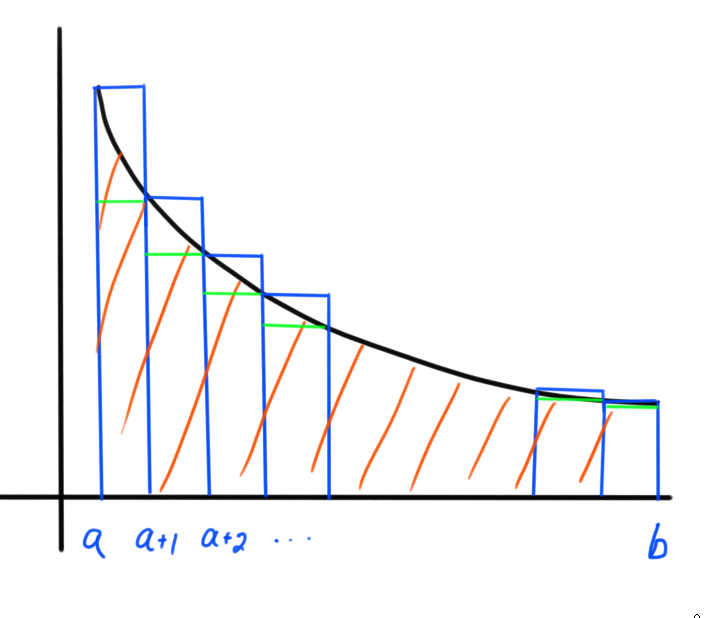
\includegraphics[scale=0.3]{integrals_and_sums}
     \end{figure}
    
    $\sum\limits_{k=a}^b f(k) - \int\limits_a^b \le \sum\limits_{k=a}^b - \sum\limits_{k=a-1}^b = f(a)$ (аналогично $f(b) = \sum\limits_{k=a}^b - \sum\limits_{k=a}^{b-1}$)

\end{proof}
\begin{theorem}[интегральный признак сходимости ряда]
    Пусть $f\!:[1, +\infty) \to \R$ неотрицательная, монотонно убывающая. 

    Тогда  $\sum\limits_{n=1}^\infty f(n)$ и  $\int\limits_1^\infty f(x) \mathrm{d}x$ ведут себя одинаково.
\end{theorem}
\begin{proof}
    По предыдущей теореме $S_n \coloneqq \sum\limits_{k=1}^n f(k) \ge \int\limits_1^n f(x)\mathrm{d}x \ge \sum\limits_{k=2}^n f(k) = S_n - f(1)$.

    Если ряд сходится, то $S_n$ --- ограничена  $\implies \int\limits_1^n f(x)\mathrm{d}x$ ограничена $\implies F(x) = \int\limits_1^x f$ --- ограничена $\implies \int\limits_1^\infty f(x)$ сходится.

    Если  $\int$ сходится $\implies \int\limits_1^n f$ --- ограничена  $\implies S_n$ --- ограничена  $\implies$ ряд сходится.
\end{proof}
\begin{example}
     \begin{enumerate}
         \item $\sum\limits_{n=1}^\infty \frac{1}{n^p}$, $p > 0$ (иначе члены ряда $\centernot \to 0$ и ряд расходится).\\
             $f(x) = \frac{1}{x^p}$. Монотонно убывает. $\sum \frac{1}{n^p}$ и $\int\limits_1^\infty \frac{\mathrm{d}x}{x^p}$ ведут себя одинаково: сходятся при  $p > 1$.
         \item $\sum\limits_{n=2}^\infty \frac{1}{n\ln n}$. $f(x) = \frac{1}{x\ln x}$ монотонно убывает. Поэтому $\int\limits_2^\infty \frac{\mathrm{d}x}{x\ln x}$ и $\sum\limits_{n=2}^\infty \frac{1}{n \ln n}$ ведут себя одинаково. 

             Там можно посчитать интеграл (разойдется).
    \end{enumerate}
\end{example}
\begin{consequence}
    \begin{enumerate}
        \item Если $a_n > 0$ и  $a_n = \mathcal{O}(\frac{1}{n^p})$ при $p > 1$ --- ряд  $\sum a_n$ --- сходится.
        \item Если  $a_n > 0$ и  $a_n \sim \frac{c}{n^p}$, то при $p > 1$ ряд  $\sum a_n$ --- сходится, а иначе расходится.
    \end{enumerate}
\end{consequence}
%END TICKET 59

\Subsection{Знакопеременные ряды}
\begin{definition}
    $\sum a_n$ --- сходится, но не абсолютно  $=$ ряд сходится условно.
\end{definition}
\begin{theorem}[Преобразование Абеля]
    $\sum\limits_{k=1}^n a_n b_n$.  $A_k \coloneqq a_1 + a_2 + \ldots + a_k$. Хочется заменить $a_n \to A_n$.

    Формулу сложнее запомнить, чем вывести, поэтому сначала выпишем её.
\end{theorem}
\begin{proof}
    \begin{align*}
        \sum_{k=1}^n a_k b_k &= \sum_{k=1}^n (A_k - A_{k-1})b_k = \sum_{k=1}^n A_kb_k - \sum_{j=2}^n A_{j-1}b_j \overset{k=j-1}{=} \sum_{k=1}^n A_kb_k - \sum_{k=1}^{n-1}A_kb_{k+1}  = \\ &= A_nb_n + \sum_{k=1}^{n-1}A_k(b_k - b_{k+1}).
    \end{align*}
\end{proof}
\begin{theorem}[Признак Дирихле]
    \begin{enumerate}
        \item $A_n$ (частичные суммы) --- ограничены ($|A_n| \le M$),
        \item $b_n$ монотонны,
        \item  $b_n \to 0$.
    \end{enumerate}
    Тогда $\sum\limits_{n=1}^\infty a_nb_n$ --- сходится.
\end{theorem}
\begin{proof}
    \begin{align*}
    S_n \coloneqq \sum_{k=1}^n a_k b_k = \underbracket{A_nb_n}_{\mathclap{\text{огр. на б.м.}}} + \sum\limits_{k=1}^{n-1}A_k(b_k-b_{k+1})
    \end{align*}
    Надо показать, что $\sum\limits_{k=1}^\infty A_k(b_k - b_{k+1})$ --- сходится. Для этого докажем, что ряд абсолютно сходится: $\sum\limits_{k=1}^\infty |A_k||b_k - b_{k+1}|$ --- сходится. 

    Мы знаем, что $\sum\limits_{k=1}^\infty |A_k||b_k - b_{k+1}| \le \sum\limits_{k=1}^\infty M \cdot |b_k - b_{k+1}| \overset{(*)}{=} M|\sum\limits_{k=1}^\infty b_k - b_{k+1}| \le M|b_1|$.

    $(*)$ --- у нас постоянная монотонность, следовательно все слагаемые одного знака.
\end{proof}
\begin{theorem}[Признак Абеля]
    \begin{enumerate}
        \item Ряд $\sum\limits_{n=1}^\infty a_n$ --- сходится,
        \item $b_n$ --- монотонны,
        \item $b_n$ --- ограничены.
    \end{enumerate}
    Следовательно, $\sum\limits_{n=1}^\infty a_nb_n$ сходится.
\end{theorem}
\begin{proof}
    $2) + 3) \implies \exists \R \ni b \coloneqq \lim b_n$. Тогда  $\widetilde{b}_n \coloneqq b_n - b$ монотонны и  $\to 0$.

     $\sum\limits_{n=1}^\infty a_n$ --- сходится  $\implies A_n$ имеет пределе  $\implies$  $A_n$ --- ограничены.

     Тогда  $\sum\limits_{n=1}^\infty a_n \widetilde{b}_n$ --- сходится  по признаку Дирихле. $\sum\limits_{n=1}^\infty a_n \widetilde{b}_n = \sum\limits_{n=1}^\infty a_n(b_n - b) \implies \sum\limits_{n=1}^\infty a_n b_n = b\sum\limits_{n=1}^\infty a_n + \sum\limits_{n=1}^\infty a_n (b_n - b)$. 
\end{proof}
\begin{definition}
    Знакочередующийся ряд $\sum\limits_{n=1}^\infty (-1)^{n-1}a_n$,  $a_n \ge 0$.
\end{definition}
\begin{theorem}[Признак Лейбница]
    Пусть есть ряд $\sum\limits_{n=1}^\infty (-1)^{n-1} a_n$.  $a_n \ge 0$ и монотонно стремится к 0.

    Тогда ряд $\sum\limits_{n=1}^\infty (-1)^{n-1} a_n$ сходится. Более того,  $S_{2n} \le S \le S_{2n+1}$.
\end{theorem}
\begin{proof}
    $S_{2n+2} = S_{2n} + a_{2n +1} - a_{2n+2} \ge S_{2n}$. $S_{2n+3} = S_{2n+1} - a_{2n+2} + a_{2n+3} \le S_{2n+1}$.

    $[0, S_1] \supset [S_2, S_3] \supset [S_4, S_5] \supset \ldots \supset [S_{2n}, S_{2n+1}] \supset \ldots$. $S_{2n+1} - S_{2n} = a_{2n+1} \to 0$.

    Пусть  $S$ не общая точка. Тогда  $\lim S_{2n} = \lim S_{2n+1} = S$.
\end{proof}

\begin{example}[Ряд Лейбница]
    \[
           \sum\limits_{n=1}^\infty \frac{(-1)^{n-1}}{n}.
    .\] 
   \begin{align*}
       S_n&=1-\frac{1}{2} + \frac{1}{3} - \frac{1}{4} + \ldots + \frac{1}{2n-1} - \frac{1}{2n} = H_{2n} - 2(\frac{1}{2} + \frac{1}{4} + \ldots + \frac{1}{2n}) = H_{2n} - H_n = \\ 
          &= \ln 2n+ \gamma + o(1) - (\ln n + \gamma + o(1)) = \ln 2 + o(1).
   \end{align*}
\end{example}
\begin{example}
    $1 - \frac{1}{2} - \frac{1}{4} + \frac{1}{3} - \frac{1}{6} - \frac{1}{8} + \frac{1}{5} - \frac{1}{10} - \frac{1}{12} + \ldots$.

    $\widetilde{S}_3n = (1 - \frac{1}{2} - \frac{1}{4}) + (\frac{1}{3} - \frac{1}{6} - \frac{1}{8}) + (\frac{1}{5} - \frac{1}{10} - \frac{1}{12}) + \ldots + (\frac{1}{2n - 1} - \frac{1}{4n-2} - \frac{1}{4n}) = \sum\limits_{k=1}^n(\frac{1}{4k - 2} - \frac{1}{4k}) = \frac{1}{2} \sum\limits_{n=1}^n (\frac{1}{2k-1} - \frac{1}{2k}) = \frac{S_{2n}}{2} \to \frac{\ln 2}{2}$.
\end{example}
\begin{definition}
    $\vphi\!: \N \to \N$ --- биекция $\sum\limits_{n=1}^\infty a_{\vphi(n)}$ --- перестановка ряда.
\end{definition}
\begin{theorem}
    Если $\sum\limits_{n=1}^\infty a_n$ абсолютно сходится, то  $\sum\limits_{n=1}^\infty a_{\vphi(n)} = \sum\limits_{n=1}^\infty a_n$.
\end{theorem}
\begin{proof}
    \begin{enumerate}
        \item $a_n \ge 0$. $S_n \coloneqq \sum\limits_{k=1}^n a_k \le S \coloneqq \sum\limits_{k=1}^\infty a_k$.

            $\widetilde{S}_n \coloneqq \sum\limits_{k=1}^n a_{\vphi(k)} \le S_{\max{\vphi(1), \ldots, \vphi(n)}} \le S \implies \lim \widetilde{S}_n \le S \implies \widetilde{S} \le S$.
        \item $a_n \in \R$.  $a_n = (a_n)_+ - (a_n)_-$, где $(a)_+ \coloneqq \max\{a, 0\}, (a)_- \coloneqq \max\{-a, 0\}$.  $|a_n| = (a)_- + (a)_+ \ge (a_n)_\pm \ge 0$.

            Если $\sum |a_n|$ --- сходится, то  $\sum\limits_{n=1}^\infty(a_n)_\pm $ --- сходится.  $\sum (a_{\vphi(n)})_+ = \sum (a_n)_+$ и  $\sum (a_{\vphi(n)})_- = \sum (a_n)_- \implies $ ряд сходится.
    \end{enumerate}
\end{proof}

\begin{remark}
    \begin{enumerate}
        \item Теорема верна в полном нормированном пространстве.
        \item В $\R^d$ верно обратное: если любая перестановка не меняет суммы, то ряд абсолютно сходится.
        \item Если ряд $a_n \in \R$ сходится условно, то  $\sum\limits_{n=1}^\infty (a_n)_+ = \sum\limits_{n=1}^\infty (a_n)_- = +\infty$.
             \begin{proof}
                Если $\sum (a_n)_+ < +\infty$, то  $\sum |a_n| = 2 \sum a_n - \sum (a_n)_+$ --- противоречие.

                 $|a_n| = 2(a_n)_+ - a_n$.
            \end{proof}
        \item Если $a_n \ge 0$, то $\sum a_{\vphi(n)} = \sum a_n$ верно и для расходящегося.
    \end{enumerate}
\end{remark}
\begin{theorem}[Теорема Римана]
    Пусть $\sum\limits_{n=1}^\infty a_n$ сходится условно, тогда  $\forall s \in \overline{\R}$ найдется такая перестановка, что  $\sum\limits_{n=1}^\infty a_{\vphi(n)} = s$.

    Так же существует перестановка, для которой нет суммы.
\end{theorem}
\begin{proof}
    Запишем сумму $a_1 + a_2 + \ldots$. Сотрем все отрицательные слагаемые: $b_1 + b_2 + \ldots = \sum (a_n)_+ = +\infty$. Сотрем все положительные: $c_1 + c_2 + \ldots = \sum (a_n)_- = +\infty$.
     \begin{enumerate}
         \item Случай $s \in \R$.  $b_1 + b_2 + \ldots + b_n > s \ge b_1 + b_2  + \ldots + b_{n-1}$.

             Теперь будем набирать $c_i$, пока сумму больше  $s$. Потом снова начнем набирать  $b$\ldots

             Обозначим за $S_i$ сумму на  $i$-ом слагаемом. Тогда знаем, что  $a_n \to 0$.  $S_1 > S \ge S_1 - b_{n_1}$, $S_2 + c_{m_1} \ge S > S_2$, $S_3 > S \ge S_3 - b_{n_2}$, $S_4 + c_{m_2} \ge S > S_4$.

             $S_{2n+1} > S \ge S_{2n+1} - s_{n_k}$. $S + b_{n_k} \ge S_{2k+1} > S$. 
         \item Случай $\pm \infty$.

             Очев + упражнение.
         \item Случай безпредела. 

             Ежу понятно.
    \end{enumerate}
\end{proof}
\begin{theorem}[Теорема Коши о произведении рядов]
    Пусть $A \coloneqq \sum\limits_{n=1}^\infty a_n$ и  $B \coloneqq \sum\limits_{n=1}^\infty b_n$ и ряды абсолютно сходятся.

    Тогда ряд, составленный из  $a_kb_n$ в произвольном порядке абсолютно сходится и его сумма  $AB$.
\end{theorem}
\begin{proof}
    $A^* \coloneqq \sum\limits_{n=1}^\infty |a_n|, A_n^* \coloneqq \sum\limits_{k=1}^n |a_k|$.  $A^*_n \le A^*, B_n^* \le B^*$.

    $S_m^*$ --- частичная сумма для рада из  $|a_kb_j|$. $S_N \le (|a_1| + |a_2| + \ldots + |a_n|)(|b_1| + |b_2| + \ldots + |b_m|) = A_n^* B_m^* \le A^* B^*$, где $n$ --- максимальный индекс у  $a_k$ в слагаемом из  $S_N^*$, $m$ --- тоже самое для  $b_k$.

    $S_N^*$ ограничены $\implies$ ряд абсолютно сходится. Можно сделать \textit{рисунок}, тогда $S_{n^2} = \sum\limits_{k=1}^n \sum\limits_{j=1}^n a_k b_j = \sum\limits_{k=1}^n a_k \sum\limits_{j=1}^n b_j = A_nB_n \to AB$. 
\end{proof}

\begin{definition}
    $\sum\limits_{n=1}^\infty a_n$ и $\sum\limits_{n=1}^\infty b_n$ произведение этих рядов --- ряд  $\sum\limits_{n=1}^\infty c_n$, где  $c_n = a_1b_n + a_2b_{n-1} + a_3b_{n-2} + \ldots + a_nb_1$.
\end{definition}
\begin{theorem}[Теорема Мертенса]
    $A = \sum\limits_{n=1}^\infty a_n, B = \sum\limits_{n=1}^\infty b_n$ --- сходится, причем один из них абсолютно.

    Тогда  $\sum\limits_{n=1}^\infty c_n$ --- сходится и его сумма  $AB$.
\end{theorem}
\begin{proof}
    Не доказывалось в курсе.
\end{proof}
\begin{remark}
    Абсолютной сходимости нет, важен порядок слагаемых.
\end{remark}
\begin{remark}
    Обычной сходимости не хватает.
\end{remark}
\begin{example}
    $\sum\limits_{n=1}^\infty \frac{(-1)^{n-1}}{\sqrt{n}}$ сходится по признаку Лейбница.

    $a_n = b_n = \frac{(-1)^{n-1}}{\sqrt{n}}$. \[c_n = (-1)^{n-1}(\underbrace{\frac{1}{\sqrt{n}} + \frac{1}{\sqrt{2}}\frac{1}{\sqrt{n-1}} + \ldots + \frac{1}{\sqrt{n}}1}_{\ge n \cdot \frac{1}{\sqrt{n}} \frac{1}{\sqrt{n}}}).\]
    А значит $|c_n| \ge 1$, а необходимое условие сходимости отсутствует. 
\end{example}
\begin{theorem}[Теорема Абеля]
    $A = \sum\limits_{n=1}^\infty a_n, B = \sum\limits_{n=1}^\infty b_n$ и  $C = \sum\limits_{n=1}^\infty c_n$ ---  произведения рядов.

    Если все три ряда сходятся, то  $AB=C$.
\end{theorem}
\begin{lemma}
    Пусть $x_n \to x$ и  $y_n \to y$. Тогда:
     \[
    \frac{x_1y_n + x_2y_{n-1} + \ldots + x_ny_1}{n} \to xy
    .\] 
\end{lemma}
\begin{proof}[Доказательство леммы]
    Случай $y=0$. Надо доказать, что $x_1y_n + \ldots + x_ny_1 = o(n)$. $|x_n| \le M, |y_n| \le M$. $\forall \eps > 0 \exists N\!: |y_n| \le \eps$ при $n \ge N$.

    Тогда в сумму все слагаемые с  $y_n$, где  $n \ge N$ будут $\le \eps M$, а первые $N$ ---  $\le M^2$. Тогда сумма $\frac{|\ldots|}{n} < \eps M + \frac{NM^2}{n} < 2\eps M$ при больших $n$.

    Случай  $y_n \equiv y$. Тогда сумма $\frac{\ldots}{n} = y \frac{x_1 + x_2 + \ldots + x_n}{n} \to xy$ по теореме Штольца.

    Общий случай: $y_n = y + \widetilde{y_n}, y_n \to 0$. Тогда сумма с  $\widetilde{y_n}$ стремится к нулю, а, следовательно исходная стремится к  $xy$.
\end{proof}
\begin{proof}[Доказательство теоремы]
    Рассмотрим $AB \leftarrow \frac{A_1 B_n + A_2 B_{n-1} + \ldots + A_nB_2}{n} = \frac{C_1 + C_2 + \ldots + C_n}{n} \to C$
\end{proof}
\Subsection{Бесконечные произведения}
\begin{definition}
    $\prod\limits_{k=1}^\infty b_k$, сходящийся, если  $\exists \lim P_n$, он конечен и  $\neq 0$.
\end{definition}
\begin{example}
    \begin{enumerate}
        \item $\prod\limits_{k=2}^\infty \left(1-\frac{1}{k^2}\right)$. Оно очевидным образом равно $\frac{1}{2}$.
        \item $\prod_{n=1}^\infty(1 - \frac{1}{4n^2}) = \frac{1 \cdot 3 \cdot 3 \cdot 5 \cdot 5 \cdot 7 \cdot \ldots \cdot (2n-1)(2n+1)}{2^2 4^2 6^2} = \frac{((2n-1)!!)^2(2n+1)}{((2n)!!)^2} \to \frac{2}{\pi}$
    \end{enumerate}
\end{example}
\begin{properties}
    \begin{enumerate}
        \item Добавление / выкидывание конечного числа ненулевых сомножителей не влияет на сходимость.
        \item Если  $\prod\limits_{k=1}^\infty b_k$ --- сходится, то  $\lim b_k = 1$.
             \begin{proof}
                $b_n = \frac{P_n}{P_{n-1}} \to \frac{P}{P} = 1$, так как $P \neq 0$ и  $\infty$.
            \end{proof}
        \item У сходящегося произведения начиная с некоторого места все множители $>0$. 
        \item  $\prod\limits_{n=1}^\infty b_n$ для  $b_n > 0$. 

             $\prod\limits_{n=1}^\infty b_n$ --- сходится  $\iff \sum\limits_{n = 0}^\infty \ln b_n$ --- сходится. Причем произведение --- $\exp$ от суммы.
\begin{proof}
    $P_n = \prod\limits_{k=1}^n b_k$.  $\ln P_n = \sum\limits_{k=1}^n \ln b_k \eqqcolon S_n$.

     $P_n$ имеет предел из  $(0; +\infty) \iff \ln P_n = S_n$ --- имеет конечный  $\lim \iff \sum \ln b_n$ --- сходящийся.
\end{proof}

    \end{enumerate}
\end{properties}
\begin{example}
    $\prod\limits_{n=1}^\infty \frac{p_n}{p_n - 1} = \prod\limits_{n=1}^\infty \sum\limits_{j=0}^\infty \frac{1}{p_n^j}$ --- где $p_n$ ---  $n$-ое простое число.

     $\prod\limits_{k=1}^n \frac{p_k}{p_k - 1} \ge H_n$.


     $\prod\limits_{k=1}^n \frac{p_k}{p_k - 1} = \prod_{k=1}^n \frac{1}{1-\frac{1}{p_k}} > \prod\limits_{k=1}^n \sum\limits_{j=0}^n \frac{1}{p_k^j} = \sum \frac{1}{p_1^{\alpha_1} \ldots p_n^{\alpha_n}} > \sum\limits_{k=1}^n \frac{1}{k} = H_n \to \infty$.
\end{example}
\begin{theorem}
    $\sum\limits_{n=1}^\infty \frac{1}{p_n}$ --- расходится. Более того $\sum\limits_{k=1}^n \frac{1}{p_k} \ge \ln \ln n - 2$.
\end{theorem}
\begin{proof}
    $\sum\limits_{k=1}^n \frac{1}{1-\frac{1}{p_k}} > H_n \implies \sum\limits_{k=1}^n \ln(\frac{1}{1-\frac{1}{p_k}}) > \ln H_n > \ln \ln n$.

    Очевидно (нет), что $\ln(1-x) \ge -x -x^2$.

    Тогда $\sum\limits_{k=1}^n \ln(\frac{1}{1-\frac{1}{p_k}}) \le \sum\limits_{k=1}^n \frac{1}{p_k} + \sum\limits_{k=1}^n \frac{1}{p_k^2}$
\end{proof}
\begin{remark}
    \[
    \sum\limits_{k=1}^n \frac{1}{p_k} = \ln \ln n + O(1).
    .\] 
\end{remark}

\end{document}
